%% bare_jrnl_compsoc.tex
%% V1.4b
%% 2015/08/26
%% by Michael Shell
%% See:
%% http://www.michaelshell.org/
%% for current contact information.
%%
%% This is a skeleton file demonstrating the use of IEEEtran.cls
%% (requires IEEEtran.cls version 1.8b or later) with an IEEE
%% Computer Society journal paper.
%%
%% Support sites:
%% http://www.michaelshell.org/tex/ieeetran/
%% http://www.ctan.org/pkg/ieeetran
%% and
%% http://www.ieee.org/

%%*************************************************************************
%% Legal Notice:
%% This code is offered as-is without any warranty either expressed or
%% implied; without even the implied warranty of MERCHANTABILITY or
%% FITNESS FOR A PARTICULAR PURPOSE! 
%% User assumes all risk.
%% In no event shall the IEEE or any contributor to this code be liable for
%% any damages or losses, including, but not limited to, incidental,
%% consequential, or any other damages, resulting from the use or misuse
%% of any information contained here.
%%
%% All comments are the opinions of their respective authors and are not
%% necessarily endorsed by the IEEE.
%%
%% This work is distributed under the LaTeX Project Public License (LPPL)
%% ( http://www.latex-project.org/ ) version 1.3, and may be freely used,
%% distributed and modified. A copy of the LPPL, version 1.3, is included
%%
%% in the base LaTeX documentation of all distributions of LaTeX released
%% 2003/12/01 or later.
%% Retain all contribution notices and credits.
%% ** Modified files should be clearly indicated as such, including  **
%% ** renaming them and changing author support contact information. **
%%*************************************************************************


% *** Authors should verify (and, if needed, correct) their LaTeX system  ***
% *** with the testflow diagnostic prior to trusting their LaTeX platform ***
% *** with production work. The IEEE's font choices and paper sizes can   ***
% *** trigger bugs that do not appear when using other class files.       ***                          ***
% The testflow support page is at:
% http://www.michaelshell.org/tex/testflow/


\documentclass[10pt,journal,compsoc]{IEEEtran}
%
% If IEEEtran.cls has not been installed into the LaTeX system files,
% manually specify the path to it like:
% \documentclass[10pt,journal,compsoc]{../sty/IEEEtran}





% Some very useful LaTeX packages include:
% (uncomment the ones you want to load)


% *** MISC UTILITY PACKAGES ***
%
%\usepackage{ifpdf}
% Heiko Oberdiek's ifpdf.sty is very useful if you need conditional
% compilation based on whether the output is pdf or dvi.
% usage:
% \ifpdf
%   % pdf code
% \else
%   % dvi code
% \fi
% The latest version of ifpdf.sty can be obtained from:
% http://www.ctan.org/pkg/ifpdf
% Also, note that IEEEtran.cls V1.7 and later provides a builtin
% \ifCLASSINFOpdf conditional that works the same way.
% When switching from latex to pdflatex and vice-versa, the compiler may
% have to be run twice to clear warning/error messages.






% *** CITATION PACKAGES ***
%
\ifCLASSOPTIONcompsoc
  % IEEE Computer Society needs nocompress option
  % requires cite.sty v4.0 or later (November 2003)
  \usepackage[nocompress]{cite}
\else
  % normal IEEE
  \usepackage{cite}
\fi

% cite.sty was written by Donald Arseneau
% V1.6 and later of IEEEtran pre-defines the format of the cite.sty package
% \cite{} output to follow that of the IEEE. Loading the cite package will
% result in citation numbers being automatically sorted and properly
% "compressed/ranged". e.g., [1], [9], [2], [7], [5], [6] without using
% cite.sty will become [1], [2], [5]--[7], [9] using cite.sty. cite.sty's
% \cite will automatically add leading space, if needed. Use cite.sty's
% noadjust option (cite.sty V3.8 and later) if you want to turn this off
% such as if a citation ever needs to be enclosed in parenpaper.
% cite.sty is already installed on most LaTeX systems. Be sure and use
% version 5.0 (2009-03-20) and later if using hyperref.sty.
% The latest version can be obtained at:
% http://www.ctan.org/pkg/cite
% The documentation is contained in the cite.sty file itself.
%
% Note that some packages require special options to format as the Computer
% Society requires. In particular, Computer Society  papers do not use
% compressed citation ranges as is done in typical IEEE papers
% (e.g., [1]-[4]). Instead, they list every citation separately in order
% (e.g., [1], [2], [3], [4]). To get the latter we need to load the cite
% package with the nocompress option which is supported by cite.sty v4.0
% and later. Note also the use of a CLASSOPTION conditional provided by
% IEEEtran.cls V1.7 and later.






% *** GRAPHICS RELATED PACKAGES ***
%
\ifCLASSINFOpdf
   \usepackage[pdftex]{graphicx}
  % declare the path(s) where your graphic files are
  \graphicspath{{figures/}}
    % and their extensions so you won't have to specify these with
  % every instance of \includegraphics
   \DeclareGraphicsExtensions{.pdf,.jpeg,.png}
\else
  % or other class option (dvipsone, dvipdf, if not using dvips). graphicx
  % will default to the driver specified in the system graphics.cfg if no
  % driver is specified.
  % \usepackage[dvips]{graphicx}
  % declare the path(s) where your graphic files are
  % \graphicspath{{../eps/}}
  % and their extensions so you won't have to specify these with
  % every instance of \includegraphics
  % \DeclareGraphicsExtensions{.eps}
\fi
% graphicx was written by David Carlisle and Sebastian Rahtz. It is
% required if you want graphics, photos, etc. graphicx.sty is already
% installed on most LaTeX systems. The latest version and documentation
% can be obtained at: 
% http://www.ctan.org/pkg/graphicx
% Another good source of documentation is "Using Imported Graphics in
% LaTeX2e" by Keith Reckdahl which can be found at:
% http://www.ctan.org/pkg/epslatex
%
% latex, and pdflatex in dvi mode, support graphics in encapsulated
% postscript (.eps) format. pdflatex in pdf mode supports graphics
% in .pdf, .jpeg, .png and .mps (metapost) formats. Users should ensure
% that all non-photo figures use a vector format (.eps, .pdf, .mps) and
% not a bitmapped formats (.jpeg, .png). The IEEE frowns on bitmapped formats
% which can result in "jaggedy"/blurry rendering of lines and letters as
% well as large increases in file sizes.
%
% You can find documentation about the pdfTeX application at:
% http://www.tug.org/applications/pdftex


\usepackage{float}
\usepackage{colortbl}
\usepackage[table*]{xcolor}
\xdefinecolor{gray95}{gray}{0.65}
\xdefinecolor{gray25}{gray}{0.8}
\xdefinecolor{blizzardblue}{rgb}{0.67,0.67,0.67}
%\usepackage{booktabs,siunitx}


% *** MATH PACKAGES ***
%
\usepackage{amsmath}
\usepackage{amsfonts}
% A popular package from the American Mathematical Society that provides
% many useful and powerful commands for dealing with mathematics.
%
% Note that the amsmath package sets \interdisplaylinepenalty to 10000
% thus preventing page breaks from occurring within multiline equations. Use:
%\interdisplaylinepenalty=2500
% after loading amsmath to restore such page breaks as IEEEtran.cls normally
% does. amsmath.sty is already installed on most LaTeX systems. The latest
% version and documentation can be obtained at:
% http://www.ctan.org/pkg/amsmath





% *** SPECIALIZED LIST PACKAGES ***
%
\usepackage{algorithm}
%\usepackage{algorithmic}
\usepackage[noend]{algpseudocode}
\makeatletter
\def\BState{\State\hskip-\ALG@thistlm}
\makeatother

%\algnewcommand\algorithmicforeach{\textbf{for each}}
%\algdef{S}[FOR]{ForEach}[1]{\algorithmicforeach\ #1\ \algorithmicdo}

% algorithmic.sty was written by Peter Williams and Rogerio Brito.
% This package provides an algorithmic environment fo describing algorithms.
% You can use the algorithmic environment in-text or within a figure
% environment to provide for a floating algorithm. Do NOT use the algorithm
% floating environment provided by algorithm.sty (by the same authors) or
% algorithm2e.sty (by Christophe Fiorio) as the IEEE does not use dedicated
% algorithm float types and packages that provide these will not provide
% correct IEEE style captions. The latest version and documentation of
% algorithmic.sty can be obtained at:
% http://www.ctan.org/pkg/algorithms
% Also of interest may be the (relatively newer and more customizable)
% algorithmicx.sty package by Szasz Janos:
% http://www.ctan.org/pkg/algorithmicx




% *** ALIGNMENT PACKAGES ***
%
\usepackage{array}
% Frank Mittelbach's and David Carlisle's array.sty patches and improves
% the standard LaTeX2e array and tabular environments to provide better
% appearance and additional user controls. As the default LaTeX2e table
% generation code is lacking to the point of almost being broken with
% respect to the quality of the end results, all users are strongly
% advised to use an enhanced (at the very least that provided by array.sty)
% set of table tools. array.sty is already installed on most systems. The
% latest version and documentation can be obtained at:
% http://www.ctan.org/pkg/array


% IEEEtran contains the IEEEeqnarray family of commands that can be used to
% generate multiline equations as well as matrices, tables, etc., of high
% quality.




% *** SUBFIGURE PACKAGES ***
%\ifCLASSOPTIONcompsoc
  \usepackage[caption=false,font=footnotesize,labelfont=sf,textfont=sf]{subfig}
%\else
 % \usepackage[caption=false,font=footnotesize]{subfig}
%\fi
% subfig.sty, written by Steven Douglas Cochran, is the modern replacement
% for subfigure.sty, the latter of which is no longer maintained and is
% incompatible with some LaTeX packages including fixltx2e. However,
% subfig.sty requires and automatically loads Axel Sommerfeldt's caption.sty
% which will override IEEEtran.cls' handling of captions and this will result
% in non-IEEE style figure/table captions. To prevent this problem, be sure
% and invoke subfig.sty's "caption=false" package option (available since
% subfig.sty version 1.3, 2005/06/28) as this is will preserve IEEEtran.cls
% handling of captions.
% Note that the Computer Society format requires a sans serif font rather
% than the serif font used in traditional IEEE formatting and thus the need
% to invoke different subfig.sty package options depending on whether
% compsoc mode has been enabled.
%
% The latest version and documentation of subfig.sty can be obtained at:
% http://www.ctan.org/pkg/subfig




% *** FLOAT PACKAGES ***
%
%\usepackage{fixltx2e}
% fixltx2e, the successor to the earlier fix2col.sty, was written by
% Frank Mittelbach and David Carlisle. This package corrects a few problems
% in the LaTeX2e kernel, the most notable of which is that in current
% LaTeX2e releases, the ordering of single and double column floats is not
% guaranteed to be preserved. Thus, an unpatched LaTeX2e can allow a
% single column figure to be placed prior to an earlier double column
% figure.
% Be aware that LaTeX2e kernels dated 2015 and later have fixltx2e.sty's
% corrections already built into the system in which case a warning will
% be issued if an attempt is made to load fixltx2e.sty as it is no longer
% needed.
% The latest version and documentation can be found at:
% http://www.ctan.org/pkg/fixltx2e


%\usepackage{stfloats}
% stfloats.sty was written by Sigitas Tolusis. This package gives LaTeX2e
% the ability to do double column floats at the bottom of the page as well
% as the top. (e.g., "\begin{figure*}[!b]" is not normally possible in
% LaTeX2e). It also provides a command:
%\fnbelowfloat
% to enable the placement of footnotes below bottom floats (the standard
% LaTeX2e kernel puts them above bottom floats). This is an invasive package
% which rewrites many portions of the LaTeX2e float routines. It may not work
% with other packages that modify the LaTeX2e float routines. The latest
% version and documentation can be obtained at:
% http://www.ctan.org/pkg/stfloats
% Do not use the stfloats baselinefloat ability as the IEEE does not allow
% \baselineskip to stretch. Authors submitting work to the IEEE should note
% that the IEEE rarely uses double column equations and that authors should try
% to avoid such use. Do not be tempted to use the cuted.sty or midfloat.sty
% packages (also by Sigitas Tolusis) as the IEEE does not format its papers in
% such ways.
% Do not attempt to use stfloats with fixltx2e as they are incompatible.
% Instead, use Morten Hogholm'a dblfloatfix which combines the features
% of both fixltx2e and stfloats:
%
% \usepackage{dblfloatfix}
% The laest version can be found at:
% http://www.ctan.org/pkg/dblfloatfix

\usepackage{caption}% http://ctan.org/pkg/caption
\captionsetup[table]{format=plain,labelformat=simple,labelsep=period}%

%\ifCLASSOPTIONcaptionsoff
 % \usepackage[nomarkers]{endfloat}
 %\let\MYoriglatexcaption\caption
 %\renewcommand{\caption}[2][\relax]{\MYoriglatexcaption[#2]{#2}}
%\fi
% endfloat.sty was written by James Darrell McCauley, Jeff Goldberg and 
% Axel Sommerfeldt. This package may be useful when used in conjunction with 
% IEEEtran.cls'  captionsoff option. Some IEEE journals/societies require that
% submissions have lists of figures/tables at the end of the paper and that
% figures/tables without any captions are placed on a page by themselves at
% the end of the document. If needed, the draftcls IEEEtran class option or
% \CLASSINPUTbaselinestretch interface can be used to increase the line
% spacing as well. Be sure and use the nomarkers option of endfloat to
% prevent endfloat from "marking" where the figures would have been placed
% in the text. The two hack lines of code above are a slight modification of
% that suggested by in the endfloat docs (section 8.4.1) to ensure that
% the full captions always appear in the list of figures/tables - even if
% the user used the short optional argument of \caption[]{}.
% IEEE papers do not typically make use of \caption[]'s optional argument,
% so this should not be an issue. A similar trick can be used to disable
% captions of packages such as subfig.sty that lack options to turn off
% the subcaptions:
% For subfig.sty:
% \let\MYorigsubfloat\subfloat
% \renewcommand{\subfloat}[2][\relax]{\MYorigsubfloat[]{#2}}
% However, the above trick will not work if both optional arguments of
% the \subfloat command are used. Furthermore, there needs to be a
% description of each subfigure *somewhere* and endfloat does not add
% subfigure captions to its list of figures. Thus, the best approach is to
% avoid the use of subfigure captions (many IEEE journals avoid them anyway)
% and instead reference/explain all the subfigures within the main caption.
% The latest version of endfloat.sty and its documentation can obtained at:
% http://www.ctan.org/pkg/endfloat
%
% The IEEEtran \ifCLASSOPTIONcaptionsoff conditional can also be used
% later in the document, say, to conditionally put the References on a 
% page by themselves.




% *** PDF, URL AND HYPERLINK PACKAGES ***
%
\usepackage{url}
% url.sty was written by Donald Arseneau. It provides better support for
% handling and breaking URLs. url.sty is already installed on most LaTeX
% systems. The latest version and documentation can be obtained at:
% http://www.ctan.org/pkg/url
% Basically, \url{my_url_here}.





% *** Do not adjust lengths that control margins, column widths, etc. ***
% *** Do not use packages that alter fonts (such as pslatex).         ***
% There should be no need to do such things with IEEEtran.cls V1.6 and later.
% (Unless specifically asked to do so by the journal or conference you plan
% to submit to, of course. )
\newcommand{\Fig}[1]{Fig.~\ref{#1}}
\newcommand{\Figure}[1]{Figure~\ref{#1}}
\newcommand{\Eq}[1]{(\ref{#1})}

% correct bad hyphenation here
\hyphenation{op-tical net-works semi-conduc-tor}


\begin{document}
%
% paper title
% Titles are generally capitalized except for words such as a, an, and, as,
% at, but, by, for, in, nor, of, on, or, the, to and up, which are usually
% not capitalized unless they are the first or last word of the title.
% Linebreaks \\ can be used within to get better formatting as desired.
% Do not put math or special symbols in the title.
%\title{Towards a Planning and Design of Fog Networks}
\title{Heuristic Algorithms for Planning and Designing Computation Offloading~Networks -- Fog Networks}
%
%
% author names and IEEE memberships
% note positions of commas and nonbreaking spaces ( ~ ) LaTeX will not break
% a structure at a ~ so this keeps an author's name from being broken across
% two lines.
% use \thanks{} to gain access to the first footnote area
% a separate \thanks must be used for each paragraph as LaTeX2e's \thanks
% was not built to handle multiple paragraphs
%
%
%\IEEEcompsocitemizethanks is a special \thanks that produces the bulleted
% lists the Computer Society journals use for "first footnote" author
% affiliations. Use \IEEEcompsocthanksitem which works much like \item
% for each affiliation group. When not in compsoc mode,
% \IEEEcompsocitemizethanks becomes like \thanks and
% \IEEEcompsocthanksitem becomes a line break with idention. This
% facilitates dual compilation, although admittedly the differences in the
% desired content of \author between the different types of papers makes a
% one-size-fits-all approach a daunting prospect. For instance, compsoc 
% journal papers have the author affiliations above the "Manuscript
% received ..."  text while in non-compsoc journals this is reversed. Sigh.

\author{Decheng~Zhang, %~\IEEEmembership{Member,~IEEE,}
        Faisal~Haider, %~\IEEEmembership{Fellow,~OSA,}
        Marc St-Hilaire %
        and~Christian~Makaya%,~\IEEEmembership{Life~Fellow,~IEEE}% <-this % stops a space

}

% note the % following the last \IEEEmembership and also \thanks - 
% these prevent an unwanted space from occurring between the last author name
% and the end of the author line. i.e., if you had this:
% 
% \author{....lastname \thanks{...} \thanks{...} }
%                     ^------------^------------^----Do not want these spaces!
%
% a space would be appended to the last name and could cause every name on that
% line to be shifted left slightly. This is one of those "LaTeX things". For
% instance, "\textbf{A} \textbf{B}" will typeset as "A B" not "AB". To get
% "AB" then you have to do: "\textbf{A}\textbf{B}"
% \thanks is no different in this regard, so shield the last } of each \thanks
% that ends a line with a % and do not let a space in before the next \thanks.
% Spaces after \IEEEmembership other than the last one are OK (and needed) as
% you are supposed to have spaces between the names. For what it is worth,
% this is a minor point as most people would not even notice if the said evil
% space somehow managed to creep in.



% The paper headers
\markboth{Journal of Internet of Things Class Files,~Vol.~14, No.~8, June~2018}%
{Shell \MakeLowercase{\textit{et al.}}: Bare Demo of IEEEtran.cls for Computer Society Journals}
% The only time the second header will appear is for the odd numbered pages
% after the title page when using the twoside option.
% 
% *** Note that you probably will NOT want to include the author's ***
% *** name in the headers of peer review papers.                   ***
% You can use \ifCLASSOPTIONpeerreview for conditional compilation here if
% you desire.



% The publisher's ID mark at the bottom of the page is less important with
% Computer Society journal papers as those publications place the marks
% outside of the main text columns and, therefore, unlike regular IEEE
% journals, the available text space is not reduced by their presence.
% If you want to put a publisher's ID mark on the page you can do it like
% this:
%\IEEEpubid{0000--0000/00\$00.00~\copyright~2015 IEEE}
% or like this to get the Computer Society new two part style.
%\IEEEpubid{\makebox[\columnwidth]{\hfill 0000--0000/00/\$00.00~\copyright~2015 IEEE}%
%\hspace{\columnsep}\makebox[\columnwidth]{Published by the IEEE Computer Society\hfill}}
% Remember, if you use this you must call \IEEEpubidadjcol in the second
% column for its text to clear the IEEEpubid mark (Computer Society jorunal
% papers don't need this extra clearance.)



% use for special paper notices
%\IEEEspecialpapernotice{(Invited Paper)}



% for Computer Society papers, we must declare the abstract and index terms
% PRIOR to the title within the \IEEEtitleabstractindextext IEEEtran
% command as these need to go into the title area created by \maketitle.
% As a general rule, do not put math, special symbols or citations
% in the abstract or keywords.
\IEEEtitleabstractindextext{%
\begin{abstract}
%As a promising computing architecture, fog computing has attracted a lot of attention from industry and research communities in recent years. 

With a huge number of heterogeneous and distributed devices performing computational and storage tasks between the cloud and users, fog computing can be an answer to the surging challenges in today's networks. However, due to the decentralized and heterogeneous nature of fog networks, planning a fog network can be a complicated and challenging task. To deal with this problem, we first propose a multi-objective mathematical model that simultaneously deals with the fog node placement, fog node dimensioning and demand routing. The model optimizes the tradeoff front (i.e. Pareto front) between capital expenditure and network delay in dual objective functions. Then, we analyze the performance of an exact algorithm (branch and bound) and two evolutionary algorithms (NSGA-II and SMPSO) on this problem, showing that the evolutionary algorithms offer a good balance between the Pareto optimality and computation time efficiency. Inspired by the existing evolutionary algorithms, we proposed a new evolutionary algorithm, named Particle Swarm Optimized Non-dominated Sorting Genetic Algorithm (PSONSGA), which combines the convergence efficiency from NSGA-II and the searching efficiency from SMPSO.  
The results demonstrate that the evolutionary algorithms are highly efficient compared to the exact algorithm. Among the three evolutionary algorithms, the algorithm we proposed (PSONSGA) gives the best Pareto front solutions, which shows the good convergence to the true optimal front and the evenly distributing property. The proposed algorithm can be a valuable planning tool for the upcoming deployment of fog networks.
\end{abstract}

% Note that keywords are not normally used for peerreview papers.
\begin{IEEEkeywords}
Computation Offloading, Fog Computing, Network Planning, Multi-Objective, Modular Facility Location, Evolutionary Algorithm, Heuristic.
\end{IEEEkeywords}}


% make the title area
\maketitle


% To allow for easy dual compilation without having to reenter the
% abstract/keywords data, the \IEEEtitleabstractindextext text will
% not be used in maketitle, but will appear (i.e., to be "transported")
% here as \IEEEdisplaynontitleabstractindextext when the compsoc 
% or transmag modes are not selected <OR> if conference mode is selected 
% - because all conference papers position the abstract like regular
% papers do.
\IEEEdisplaynontitleabstractindextext
% \IEEEdisplaynontitleabstractindextext has no effect when using
% compsoc or transmag under a non-conference mode.



% For peer review papers, you can put extra information on the cover
% page as needed:
% \ifCLASSOPTIONpeerreview
% \begin{center} \bfseries EDICS Category: 3-BBND \end{center}
% \fi
%
% For peerreview papers, this IEEEtran command inserts a page break and
% creates the second title. It will be ignored for other modes.
\IEEEpeerreviewmaketitle



\IEEEraisesectionheading{\section{Introduction}\label{sec:introduction}}
% Computer Society journal (but not conference!) papers do something unusual
% with the very first section heading (almost always called "Introduction").
% They place it ABOVE the main text! IEEEtran.cls does not automatically do
% this for you, but you can achieve this effect with the provided
% \IEEEraisesectionheading{} command. Note the need to keep any \label that
% is to refer to the section immediately after \section in the above as
% \IEEEraisesectionheading puts \section within a raised box.




% The very first letter is a 2 line initial drop letter followed
% by the rest of the first word in caps (small caps for compsoc).
% 
% form to use if the first word consists of a single letter:
% \IEEEPARstart{A}{demo} file is ....
% 
% form to use if you need the single drop letter followed by
% normal text (unknown if ever used by the IEEE):
% \IEEEPARstart{A}{}demo file is ....
% 
% Some journals put the first two words in caps:
% \IEEEPARstart{T}{his demo} file is ....
% 
% Here we have the typical use of a "T" for an initial drop letter
% and "HIS" in caps to complete the first word.
\IEEEPARstart{T}{he} conventional cloud computing paradigm has been applied as a solution for delivering a diverse range of services. However, the long network distance between edge devices and remote datacenters hinders the service quality of the application, resulting in high latency, high bandwidth consumption and unreliable connectivity~\cite{Vaquero:2014:FYW:2677046.2677052}. 

Even worse is the challenges posed by the Internet of things (IoT) applications. For instance, IoT applications usually require mobility support, geo-distribution, location-awareness and low latency~\cite{bonomi2014fog}. The traditional cloud system can hardly provide these requirements and have unsolved problems in service management, connectivity and security challenges~\cite{yi2015survey}. 

To address the aforementioned challenges, Cisco proposed the concept of fog computing. The idea of fog computing is to bring computation, communication and storage closer to the end-users~\cite{yi2015survey}. In this platform, applications and workloads are run over a local micro-datacenters (named fog), instead of connecting to the remote cloud. Since services are hosted on the mini-cloud facility in the vicinity of the end users, the dispensable network hops can be eliminated thus minimizing the response time for applications. In addition, fog computing can alleviate the traffic congestion in the Internet backbone since the huge amount of traffic generated by end devices can be locally handled by the fog servers. Typically, the fog architecture can be described as shown in~\Fig{foggg}. The fog architecture is deployed as a large number of micro-datacenters, which are often distributed over a geographical region of interest. These fog nodes connect to access networks and remote clouds to provide storage and computing services without the intervention of third-parties~\cite{chiang2016fog}.

\begin{figure}[ht]
\centerline{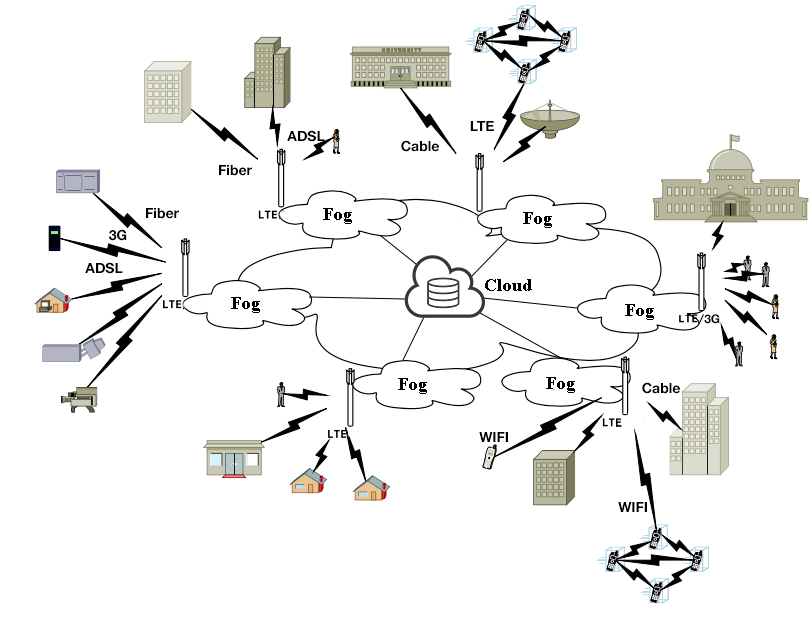
\includegraphics[width=\columnwidth]{fog-g.png}}
\caption{Typical fog network architecture} 
\label{foggg}
\end{figure}
 
The proximity offered by fog networks addresses the challenges facing today's cloud infrastructures, and enables low-latency IoT applications. However, when it comes to the planning of fog networks, considering the decentralized nature of the fog network combined with a large number of edge devices, obtaining the optimal network design can be challenging. The following factors must be taken into consideration:
\begin{itemize}
\item Fog facilities need to be highly decentralized and close to the edge devices.
\item The fog architecture needs to take into account heteromerous hardware requirements.
\item User demands need to be distributed across multiple facilities.
\item The center cloud needs to be able to connect and cooperate with the fog facilities.
\end{itemize}

%%%%%%%%%%%%%%%
%Essentially, the fog planning problem is composed of two sub-problems, each of them has been proven to be NP-hard:
%\begin{itemize}
%\item Capacitated facility location problem \cite{megiddo1983maximum,1.43} %COMMENT: Can you add a reference showing that this problem is NP-hard
%\item Resource allocation problem \cite{trove.nla.gov.au/work/12815220}%COMMENT: Can you add a reference showing that this problem is NP-hard
%\end{itemize}
%In addition, from the operator point of view, the objectives of the fog planning can be targeted to two conflicting objectives:
%\begin{itemize}
%\item Minimize capital expenditure
%\item Minimize network delay
%\end{itemize}

Therefore, an integrated framework for computation offloading, hardware resource allocation and facility provisioning has the potential to significantly improve the performance of edge network with fog computing.

%%%%REVISED
By convention, the single-objective optimization is employed in network planning. The designing process is essentially an allocation problem which maximizes the network utility function over a fixed capital expenditure constraint. 
However, in network planning, it is possible to greatly improve the network performance whilst incurring a very small increase in capital expenditure. Such compromise solutions can be easily missed using the single objective method. To obtain such optimal solution, network designers must use a form of trial and error to try different budget options. The inability to derive an analytical perspective of the problem requires the network designer to execute the single-objective optimization multiple times, which significantly increasing the computational overhead. 
In contrast, the multi-objective optimization, we adopt in this work, is more desirable for the fog network design. First, the multi-objective optimization searches the optimal set of trade-off solutions and simultaneously takes all the objectives into considerations. Hence, it can easily catch the aforementioned tradeoff solution.
Second, since the multi-objective optimization techniques attempt to find multiple non-dominated and isolated solutions in a single simulation by emphasizing multiple solutions towards Pareto-front, it greatly speeds up the optimizing process. 

%%%%%%%%%%%%%%%%%%




A recent comprehensive survey on the state-of-the-art fog research has noted that the planning and design of fog system deployment received little attention so far~\cite{mouradian2017comprehensive}. Besides, to the best of our knowledge, the joint design of computation offloading, resource allocation and facility provisioning has not been addressed in previous work. The contributions of this paper are as follows.
\begin{itemize}
\item We formulate the offloading decision, facility locating, and facility provisioning in edge networks with fog computing as an optimization problem.
\item The model formulation and optimal results obtained through MIP toolbox, can be used as benchmark for heuristic algorithm development.
\item We apply the weighted sum and exist evolutionary algorithms to solve  the multi-objective fog planning problem.
\item We propose an new evolutionary algorithm to solve the problem in an efficient and practical way.
\item Simulation results are presented to show the effectiveness of the proposed algorithm with different benchmark and comparison testing.
\end{itemize}

%To deal with this problem and provide high-performance fog system design, we propose a mathematical model in this paper, which simultaneously determines the optimal location, the capacity and the number of fog node(s) as well as the interconnection between the installed fog nodes and the cloud. 
%Since this model is a multi-objective model, we address the multi-objective functions with one exact algorithm and three approximation algorithms, and compare the results in terms of the delay, CPU time and multi-objective quality indicators. 


The remainder of the paper is organized as follows. In Section \ref{probfor}, the fog planning problem formulation is presented. In Section \ref{nphard}, the NP-hardness of the Fog Planning model is analyzed. Section \ref{alfpp} presents a comprehensive explanation of the multi-objective algorithms and optimization procedures. 
%The multi-objective algorithms include the weighted sum method, NSGA-II algorithm, SMPSO algorithm and the proposed PSONSGA algorithm. 
Numerical results are presented in Section \ref{express}, including the evaluation and comparison in terms of the solution quality and computation time. In Section \ref{relwork}, we overview some related works in the area of fog computing and distributed-cloud planning. Finally, conclusions are drawn in Section \ref{conclu}.

\section{Problem Formulation}\label{probfor}
To help understand the problem modeling, we first introduce the following basic concepts.

%\subsection{Basic Concepts}
%\textbf{Fog placement} is the process of selecting a subset of potential locations from a given candidate set and placing fog facilities at these locations.% in order to serve the requests of edge-clusters.

%\textbf{Fog dimensioning} is the process of selecting the capacity levels of fog devices and link types for each candidate site. This selection depends on the node cost, link cost and requirements of edge-clusters' demands.

\textbf{Resource demand: }In this paper, two types of resources are considered at the fog nodes: vCPU cores and memory. 
%For each fog nodes, let $C_{f_i}$ and $ M_{f_i}$ denotes the aggregate request of CPU and memory respectively. It is assumed that fog nodes are provisioned with these two type of resources. 
However, other resources can be included such as the storage and GPU units. This can be achieved by increasing the dimension of the fog profile. For any single period of time, each user-cluster generates a request consisting of vCPU, memory, and bandwidth demands. If a request can be routed to a fog node in such a way that the required vCPU, memory and link bandwidth can be satisfied, then the request is served; otherwise, the request is sent to the cloud. 

%Given the bipartite graph $G(I, J)$, the objective of the FPP is to, according to the aggregate $C_{f_i}, M_{f_i}$ (CPU demands and memory demands), choose the modular $K$ for each fog centre f and choose the link type $l, (l \in L)$ for each link. Also, each edge cluster $j \ (j \in J) $ should be served by either the fog or the cloud in a sense that the total network usage is minimized. The network usage here can be defined as end-to-end delay or weighted traffic and latency values.
\textbf{Fog type: }The fog type is an abstraction of the real-world machine servers. Different fog types are associated with different computation resources. In real-world planning, the number of fog types and fog profiles can be changed to adequate types or amounts.

\textbf{Link type: }Similarly, different link types between the fog nodes and the cloud are considered. Each link is associated with a bandwidth capacity. These links carry the traffic flow between the fog nodes and the cloud for back-end services such as data synchronizations and application management.

\textbf{Edge-cluster: }The notion of edge-cluster is used to represent an agglomeration of user requests. Typically, several users are using the cloud at the same time from a common geographical region sharing a unique IP prefix. Instead of modelling them individually, we aggregate them together as an ``edge-cluster". However, in optimization research, the request unit is named as ``user". In this paper, the terms ``user'' and ``edge-cluster" have the same meaning.
%%%REVISED
It is noteworthy that we are planning based on overall expected traffic from each ``end user'' to computation facilities. The dynamic day to day management can be done via other load balancing and resource allocation schemes which is beyond this topic and can be exploited in future research.

%\textbf{Edge-cluster routing} can be modelled as an assignment problem. After fog placement and dimensioning decisions are made, an assignment problem must be solved to optimally match edge-clusters with fog facilities.


\subsection{Assumptions}\label{assumption}
This section describes the assumptions used in this paper. To formulate the fog planning model, we assume the following information is known:  
\begin{itemize}
\item The locations of all the edge devices and the possible locations of all the fog nodes (i.e., $x$ and $y$ coordinates). For each edge device, the generated traffic is known.
\item The characteristics, i.e., memory, virtual Central Processing Unit (vCPU) of different types of fogs that may be installed in the network.
\item The bandwidth availability and the cost of each link type. The links are installed between the fog nodes and the cloud.
\item The cloud has unlimited memory and vCPU. We also assume that the cloud is located in a remote location and if a user cannot be served by the fog, it will be routed to the cloud.
\item The fog nodes send a fix ratio $\tau$ of their total traffic to the cloud. The $\tau$ here is a tunable parameter. Different applications will have a different value of $\tau$ which captures the amount of traffic that needs to be sent from the fog nodes to the cloud. The possible components of this traffic include database synchronization, data uploading, service management, etc.
\end{itemize}


%\section{FPP Formulation} \label{sec:fppf}
%In this section, we formulate the fog planning problem as the bi-objective combinatorial optimization problem. Since the building cost and total network delay are equally essential in decision making, defining a bi-objective formula and solving this model in the later chapter is a better option. The bi-objective problem defined here makes sure we have a complete idea of the whole search space of this problem. Therefore, no better option will be left out.




\subsection{Notation}

The following notation is defined based upon the information mentioned above.

\begin{enumerate}
\item Sets
\begin{itemize}
\item $ \textit{I} = \{ 1,...,i,...,m \}$, set of potential location sites. Location $m$ represents the remote cloud-centre.
\begin{itemize}
\item $c_i^{Rent}$, the renting cost for each potential location $i \in I$.
\end{itemize}
\item $\textit{J}$, set of edge device clusters that must be served by the fog nodes or the cloud. Each edge-cluster has an aggregated memory, vCPU and traffic demands.
\begin{itemize}
\item $\eta_j$, the total number of vCPU required by an edge-cluster $j \in J$.
\item $\zeta_j$, the total amount of memory required by an edge-cluster $j \in J$.
%\item $\theta_j$, the number of packets requested to the fog nodes or the cloud by a cluster of edge devices $j \in J$
\item $T_j$, the total traffic generated by an edge-cluster $j \in J$.
\item $\kappa_j$, the link speed of an edge-cluster $j \in J$.
\end{itemize}

\item $K$, set of fog types (or capacity level) that can be installed at different locations. Different fog types $k \in K$ have different amount of vCPU and memory.
\begin{itemize}
\item $\alpha^k$, the total number of vCPU available for a fog of type $k \in K$.
\item $\lambda^k$, the total amount of memory available for a fog of type $k \in K$.
\item $c_k^{Fog}$, the cost for a fog of type $k \in K$.
\end{itemize} 
%, different location can have different set of fog type, according to localized space, electricity level and policy restriction.
\item $L$, set of link types that can be installed at different locations to maintain connections to cloud datacenters. Different link types $l \in L$ have different bandwidth capacities. 
\begin{itemize}
\item $\beta^l$, the egress bandwidth upper limit for link type $l \in L$.
\item $c_l^{Link}$, the cost (\$/meter) for a link of type $l \in L$.
\end{itemize}
\end{itemize}


\item Functions
\begin{itemize}
\item $d_{ab} = Distance (\textit{a}, \textit{b})$. The euclidean distance between points \textit{a} and \textit{b}. The values of points \textit{a} and \textit{b} are the \textit{x}, \textit{y} coordinates.
\item $\gamma$, processing delay. Each router or switch in the data path adds a finite amount of delay as the packet is received, processed, and then forwarded. This includes the time taken at each layer of the Transmission Control Protocol/Internet Protocol (TCP/IP) down to the bit level layer. The processing delay depends on the hop count between user's connection to fog or cloud. The processing delay is calculated as: 
\begin{align}
\text{Processing Delay} : \gamma = r \cdot h %COMMENT: in the description above, you say that gamma is the processing delay but in the equation here, gamme is a parameter to the processing delay function...please try to make this consistent...the same applies to the other delay equations below...
\end{align}
where $r$ is the mean processing delay for each hop (switch or router) and $h$ represents the hop count.
\item $\psi$, transmission delay. The time taken for a process to send the information to the transmission medium (fiber or wire). The transmission delay depends on the link speed that is used and the packet size that is to be sent. The transmission delay is calculated as: 
\begin{align}
\text{Transmission Delay} : \psi =\sigma / \kappa
\end{align}
where $\sigma$ is the packet size (bytes) and $\kappa$ represents the link speed (bytes/sec).
\item  $\mu$, propagation delay. It equals to the time taken for the signal to propagete from the source to the destination. The propagation delay depends on the medium used. For copper wires, the speed can be approximated to 0.59 speed of light. In this paper, we use 0.59 speed of light for the speed of copper wire. The propagation delay is calculated as:  
\begin{align}
\text{Propagation Delay} : \mu = \frac{d_{ab}}{(0.59 \cdot Light\ Speed)}
\end{align}
where $d_{ab}$ is the euclidean distance between edge-cluster $a$ and fog $b$ ($km$). 

\item$D(d_{ab})$. The function $D(x)$ is the network usage descriptor. The network usage function $D(x)$ is a representation of the network usage between each user and fog facilities, which could represent the network latency experienced by users or the traffic sent to the cloud. This function is transparent to the optimization algorithm. %COMMENT: I am not sure this is clear...

In real life planning, latency is arguably the most important performance metric. A small increase in the latency can cause substantial service level degradation \cite{7833029,6678113}. Therefore, in our experiment, the network usage function $D(x)$ is modelled as the point to point delay. 

\end{itemize}
\item Decision Variables
\begin{itemize}
\item $x_{ij}$, a 0-1 variable such that $x_{ij} = 1$ if and only if the edge device cluster $j \in J$ is connected to location $i\in I $;
\item $y_{ik}$, a 0-1 variable such that $y_{ik} = 1$ if and only if the fog type $k \in K_i$ is installed at location $i \in I$;
\item $z_{il}$, a 0-1 variable such that $z_{l}=1$ if and only if the link type $l \in L$ is installed at location $i \in I $. 
\end{itemize}
\end{enumerate}


\subsection{Mathematical Model}\label{obj}
Based on the notation presented in the previous section, we can now formulate the Fog Planning Problem, denoted FPP, as follows:

Minimize Cost
\begin{equation}\label{obj1}
\begin{aligned}
\textit{Minimize}\bigg[\sum_{i=1}^{m}\sum_{k\in K} y_{ik}c^{Rent}_i +\sum_{i=1}^{m}\sum_{k\in K}  y_{ik} c^{Fog}_k +\\
\sum_{i=1}^m \sum_{l\in L} z_{il} c^{Link}_l d_{i,cloud}\bigg] %COMMENT: When you look at the output, this equation has 2 equation numbers...can you fix?
\end{aligned}
\end{equation}

Minimize Delay 
\begin{align}\label{obj2}
\textit{Minimize} \bigg[\sum_{i=1}^m\sum_{j\in J} D(d_{ij}) x_{ij}\bigg]
\end{align}

%COMMENT: What is this for? is this part of the objective function? is this a constraint? It also has no equation number...
% This is the network usage function we mentioned before. In our experiment, it represents the network delay. As we can see connecting to cloud or fog gives different delay. Since it just a detailed explain of the D(x) function, I avoid giving "equation number" on this function.

%$$
%D(d_{ab})  = 
%	\begin{cases}
%	\begin{aligned}
%	&\psi^{ToFog} + \mu^{ToFog} + \gamma^{ToFog}&\sum_{i \in I  \setminus m}x_{ij} =1&\quad\\
%	 &\textbf{ (connect to the fog)}\\
%	&\psi^{ToCloud} + \mu^{ToCloud} + \gamma^{ToCloud}&x_{mj} = 1&\quad\\
%	& \textbf{ (connect to the cloud)}\\
%	\end{aligned}
%	\end{cases}
%$$

As shown above, to achieve the maximum network performance and cost efficiency, the model simultaneously minimizes the total network delay and the total capital expenditure required to deploy the fog network.  

Both Equation \Eq{obj1} and Equation \Eq{obj2} are subject to following constraints:
\begin{align}
&\sum_{i=1}^m x_{ij} =1\quad  (\forall j \in J )\label{st1}
\end{align}
Constraints \Eq{st1} are the single source constraints. They ensure that each user connects to exactly one fog or cloud. \\
\begin{align}
&\sum_{k\in K} y_{ik} \leq1 \quad(\forall i \in I )\label{st2}
\end{align}
Constraints \Eq{st2} are the uniqueness constraints. They enforce that at most one fog node is installed at a given location.  In practice, we can install multiple servers in each location, and each server can have different hardware configurations (memory sticks, CPU, hard disk drive, GPU, etc.) To reduce the complexity, we generalize different server types and hardware combinations to a fix number of fog types. Under this assumption, each potential location can select an appropriate fog type to accommodate the workload demands. In other words, we cannot install two or more fog nodes at the same location. If the left side of Equation \Eq{st2} equals to zero, it means that the corresponding location is not selected; no fog facility will be installed at this location.\\
\begin{align}
&\sum_{l\in L} z_{il} \leq1\quad(\forall i \in I) \label{st22} %COMMENT: Do we really need this constraint? 
\end{align}
Similar to Constraints \Eq{st2}, Constraints \Eq{st22} are the link uniqueness constraints. They enforce that at most one link type can be installed at each location. If Equation \Eq{st2} equals to zero, the corresponding location is not used and therefore, no link will be installed at this location.\\
\begin{align}
& x_{ij} - \sum_{k\in K} y_{ik}\leq0  \quad(\forall i \in I,\forall j \in J)\label{st3}
\end{align}
Constraints \Eq{st3} are the openness constraints. They ensure that users can only connect to a fog that is opened/used.\\ 
\begin{align}
&\sum_{l\in L} z_{il} \leq \sum_{k\in K} y_{ik} \quad (\forall i \in I) \label{st23}
\end{align}
Constraints \Eq{st23} make sure that each installed fog node at location $i$ will be connected to the cloud.\\
\begin{align}
&\sum_{j\in J} \eta_j x_{ij} \leq \sum_{k\in K} y_{ik}\alpha^k \quad(\forall i \in I)\label{st4}
\end{align}
\begin{align}
&\sum_{j\in J} \zeta_j x_{ij} \leq \sum_{k\in K} y_{ik}\lambda^k \quad(\forall i \in I)\label{st41}
\end{align}
Constraints \Eq{st4} and \Eq{st41} are the capacity constraints for vCPU and memory at the node level. They ensure that the total resource demand does not exceed each fog node's hardware capacity. 
\begin{align}
&\sum_{j\in J} x_{ij} T_j \cdot \tau \leq \sum_{l\in L} z_{il} \beta^l\quad(\forall i \in I) \label{stl}
\end{align}
Constraints \Eq{stl} are the link capacity constraints. They state that the total bandwidth from fog site to cloud cannot exceed the egress link bandwidth upper bound.\\
\begin{align}
&x_{ij} \in \{0,1\} \quad (\forall i \in I, \forall j \in J)\label{st5}\\
& y_{ik} \in \{0,1\} \quad (\forall i \in I, \forall k \in K)\label{st6}\\
& z_{ik} \in \{0,1\} \quad (\forall i \in I, \forall k \in K)\label{st7}
\end{align}
Finally, Constraints \Eq{st5}, \Eq{st6} and \Eq{st7} define the decision variables as binary.

%%REVISED shorten the NP-hard analysis
\section{NP-Hardness}\label{nphard}
This section establishes the NP-hardness of the FPP.
The FPP has two objective functions that need to be minimized: capital expenditure and network delay. The decision variables consist of the placement and assignment decisions. %COMMENT: Try to be consistent: Sometimes, you refer to building cost, sometimes to capital expenditure...it is better if you stick to 1 term....

Essentially, this problem is a multi-objective combinatorial problem.
Two related problems in single objective optimization are K-median clustering problem and Capacitated Facility Location Problem (CFLP)
%If we relax certain conditions, there are related single-objective optimization problems that we can gain insight from.
%Suppose that we know that a certain number of fog facilities will be opened and that we relax the capacity constraints at each location. Then, the problem of assigning edge-clusters to open facilities while minimizing the total delay can be reduced to the K-median clustering problem.

%\textbf{K-median clustering problem}: Suppose there exists a bipartite graph with a bi-partition (F, C), where F is a set of facilities and C is a set of clients, and let $k$ be a positive integer specifying the number of facilities allowed to be opened. Let $c_{ij}$ be the cost of connecting client $j$ to facility $i$. The objectives are to find a subset $I \subseteq F, |I| \leq k$ of facilities that should be opened and a function $\phi: C \to I$ assigning clients to open facilities that minimize the total connecting costs \cite{Vazirani:2001:AA:500776}.

The NP-hardness of the K-median clustering problem has been proved in 1984 by Megiddo and Supowit~\cite{1984}. 
However, even if we can solve this problem using an approximation algorithm, we still have to decide a reasonable $k$ regarding to the total budget. 

%From another perspective, suppose we combine the capital expenditure and network delay into a single objective function. The objective function becomes:
%\begin{align}
%\textit{Minimize}: \ \alpha\cdot\overset{opened\ fog}{\sum} \textit{fog capital expenditure} + \\
%\beta \cdot \overset{all\ users}{\sum}\textit{network delay}\nonumber
%\end{align}
%where $\alpha$ and $\beta$ are the normalizing constants.
%Problems of this form are referred to as the capacitated facility location problem.\\

%\textbf{Capacitated Facility Location Problem (CFLP)}: Suppose there exists a bipartite graph with a bi-partition (F, C), where F is a set of facilities and C is a set of clients. A fixed cost $f_i \geq 0 $ for opening each facility $i \in F$; a capacity $u_i \geq 0 $ for each facility $i \in F$; a demand $d_j \geq 0$ for each client $j \in C$. The problem is to find a subset $I \subseteq F$, of facilities to opened as well as a assignment function $\phi: C \to I $ that assigns clients to open facilities. The objective is to minimize the total connecting cost without violating each facility's capacity constraint: $\sum_{j \in C} x_{ij} d_j \leq u_i,  \forall i \in F$~\cite{Vazirani:2001:AA:500776}. 

Megiddo and Supowit~\cite{1984} proved that exact solution of CFLP is NP-hard. Fowler el al.~\cite{FOWLER1981133} proved that when the error is small, even an approximation to this problem is NP-hard.

%Specifically, our problem needs to add a single source constraint. The reason is each users can only go to one single fog; in this regard, the problem becomes the Single-Source Capacitated Facility Location Problem (SSCFLP). In SSCFLP, deciding whether a feasible solution exists at all is NP-complete~\cite{bonn}.
%Moreover, our problem has a modular facility cost model, which provides several capacity levels of the fog facility. This transfers the model to a single-source modular capacitated facility location problem, which is a more complicated version of CFLP~\cite{bonn}.

As mentioned above, the single objective models of this problem are NP-hard and computationally complex. In fact, without an efficient approach, the multi-objective model, which combines the optimization of these two objectives in one single optimization process, can be even challenging.

\section{Algorithms for FPP}\label{alfpp}

\subsection{Exact Algorithm for FPP}
To solve the multi-objective problem, the directed thinking approach is to combine multiple objectives into one single objective. The Weighted Sum Method applies to this ideology.

\subsubsection{Weighted Sum Method}
The weighted sum approach combines multiple objective functions into a single objective function. In this combination, different objectives are given a certain weight between 0 and 1. The multi-objective problem can be combined by using the Formula \Eq{wsequation}.

\begin{align}
&min\ or\ max \bigg\{\sum_{j=1}^Q \lambda_j z^j (x) : x \in X \bigg\}\label{wsequation}\\
&0\leq \lambda_j \leq 1\\
&\sum_{j=1}^Q \lambda_j = 1
\end{align}

where $\lambda_j$ is the weight parameter assigned to each objective to capture the relative importance on a given objective. Each objective function is normalized before calculating the resultant objective function. %REVISED

%Assigning a higher (lower) weight places more (less) emphasis on this objective.% In our FPP experiment, 11 pairs of weights (with steps of 0.1) is applied to solve each problem instance.

\subsection{Approximate Algorithms for FPP}\label{sec:approximate}
In this paper, the Evolutionary Multi-objective Optimization (EMO) is applied to solve the fog planning problem. EMO is based on heuristic multi-objective optimization techniques that imitate the principles of natural selection and survival of the fittest to find near-optimal solutions. In EMO, multiple Pareto-optimal solutions are found in a single simulation by emphasizing multiple non-dominated and isolated solutions \cite{Deb:2001:MOU:559152}. %COMMENT: Fix the reference [23] - [23] appears at 2 places...
The experiment results show that neither NSGA-II nor SMPSO is capable to produce solid results with strict convergence and rich coverage. Therefore, we propose an algorithm (PSONSGA) to overcome the drawbacks of these algorithms. The experiments in next section show that our algorithm outperforms NSGA-II and SMPSO in coverage and convergence respectively.
%Comment: Be consistent in how you write NSGA-II vs NSGAII... see above and below...but check the whole document...
\subsubsection{Non-dominated Sorting Genetic Algorithm II (NSGA-II)}
NSGA-II follows the same steps as the classical GA. 
%The classical GA first initializes a population of \textit{N} individuals, then it generates offsprings by applying the crossover and mutation operations, and finally evaluates and selects the fittest solutions as output solutions. 

What differentiates NSGA-II from previous algorithms (such as VEGA and HLGA) is an intuitive invention of the fast elitist ranking procedure (Non-dominated Sorting). Using this fast ranking procedure, NSGA-II always preserves the best (higher rank in non-dominated rank and larger crowding distance) solutions inside the latest population. 
%The pseudocode of the NSGA-II algorithm is presented in Fig~\ref{nsga2}. %COMMENT: Always use the tilda before referencing figures, tables or references...it will create a constant spacing

%\begin{figure}[ht]

%\indent\fbox{%
%\begin{minipage}{\dimexpr\linewidth-2\fboxsep-2\fboxrule\relax}
%\quad
%\begin{algorithmic}[1]
%\STATE Initialize a population of $N$ individuals as the ``parent population" P 
%\WHILE{\texttt{Iteration $<$ MaxIteration}}
%	\STATE \textit{C} $\gets$ Empty\ child\ population
%	\WHILE{\texttt{the number of individuals \textit{C} in <  $N$}}
%	\STATE Select\ parent1 (by\ tournament\ selection)
%	\STATE Select\ parent2 (by\ tournament\ selection)
%	\STATE Get child1, child2 through the Binary Crossover (parent1,\ parent2)
%	\STATE Polynomial\ Mutation (child1, child2)
%	\STATE Evaluate\ child1, child2\ for their fitness values
%	\STATE Insert\ child1,\ child2\ into\ \textit{C}
%	\ENDWHILE
%	\STATE \textit{U} $\gets$ Combine\ \textit{P}\ and\ \textit{C}\ to\ get\ \textit{2N}\ individuals
%	\STATE Rank\ the\ union\ set\ \textit{U}\ using\  the non\-dominated\ sorting. %(As\ explained\ in\ \ref{nds})
%	\STATE \textit{P} $\gets$ \textit{N}\ front\ individuals\ in\ \textit{U}\ by\ the crowded\ comparison\ selector. %(As\ explained\ in\ \ref{cdc})
%\ENDWHILE
%\STATE Return the set of feasible non-dominated solutions in the latest population.
%%\EndProcedure
%\end{algorithmic}
%\label{nsga2}
%\end{minipage}% 
%}
%\caption{NSGA-II Algorithm}
%\label{nsga2}
%\end{figure}



\subsubsection{Speed-Constrained Multi-Objective Particle Swarm Optimization (SMPSO)}
Particle Swarm Optimization (proposed by J. Kennedy and R. Eberhart in~\cite{poli2017}) models the social behaviour of biological creatures through the mathematical approach.

%The pseudocode of the SMPSO algorithm is presented in Fig~\ref{SMPSO}. %COMMENT: Do you call them algorithm or figure??  if you call them figure, make sure the caption appears below the figure and not on top as it is currently the case...
SMPSO first randomly generates a set of \textit{N} initial solutions, then iteratively updates the ``solution positions" in the searching space~\cite{smpso}.
In each iteration, every particle adjusts its velocity to follow the local and global best solutions. 
%We assume that each particle $i$ is randomly assigned a position $\vec{x}_i\ (i=1, 2, ..., N)$ and a velocity $\vec{v}_i\ (i=1,2,...,N)$. The algorithm updates the particle's position by:
%\begin{equation}\label{psoposition}
%\vec{x}_i(t) = \vec{x}_i(t-1) + \vec{v}_i(t)
%\end{equation}
%The velocity function $\vec{v}_i(t)$ is given by:
%\begin{equation}\label{psospeed}
%\vec{v}_i(t) = w \cdot \vec{v}_i(t-1) + C_1 \cdot r_1 \cdot (\vec{x}_{p_i}- \vec{x}_i)+ C_2 \cdot r_2 \cdot (\vec{x}_{g_i} - \vec{x}_i)
%\end{equation}
%where $\vec{x}_i(t)$ and $\vec{v}_i(t)$ are the location and velocity of particle \textit{i} at time \textit{t}. 
%The $\vec{x}_{p_i}$ and $\vec{x}_{g_i}$ are respectively, the historical best and the global best points.
%$w$ is the inertia weight of the particle, which controls the trade-off between the global and local experience.
%$C_1$ and $C_2$ are learning factors which control the effect of the local and global best particle.
%$r_1$ and $r_2 $ add randomness between the global and local searching direction.


%\begin{figure}[ht]
%
%\indent\fbox{%
%\begin{minipage}{\dimexpr\linewidth-2\fboxsep-2\fboxrule\relax}
%\quad
%\begin{algorithmic}[1]
%\STATE Initialize a population of \textit{N} individuals as ``swarm population" \textit{S} 
%\STATE Evaluate the solutions in the ``swarm population"
%\STATE Put non-dominated solutions into an empty ``elite archive" \textit{A} 
%\WHILE{\texttt{Iteration $<$ MaxIteration}}
%	\FOR{$s \in S$}
%		\STATE Use constrained binary tournament to select a solution from the elite archive
%		\STATE Use the solution from last step as the global best particle
%		\STATE Compute the speed of \textit{s} according to the speed formula \Eq{psospeed}
%		\STATE Update the position of \textit{s} according to the speed calculated in the last step
%	\ENDFOR
%	\STATE Apply the polynomial mutation to $\tau \%$ of the population
%	\STATE Evaluate the solutions in the swarm population 
%	\STATE Insert the non-dominated solutions from $S$ to $A$.
%\ENDWHILE
%\STATE Return the set of feasible non-dominated solutions in the elite archive ($A$).
%\end{algorithmic}
%\label{SMPSO}
%\end{minipage}% 
%}
%\caption{SMPSO Algorithm}
%\label{SMPSO}
%\end{figure}


\subsection{Proposed EMO Algorithm (PSONSGA)}
Motivated by the disadvantages in NSGA-ii and SMPSO algorithms, we propose a new evolutionary algorithm called particle swarm optimized non-dominated sorting genetic algorithm (PSONSGA). PSONSGA is specifically designed to combine the searching efficiency of two different types of evolutionary algorithm (PSO and GA). More precisely, the PSONSGA algorithm follows a two-phase methodology. In the first phase, the PSO procedure is executed to preprocess the pareto solution set. Then, in the second phase, the NSGA-II procedure is employed to reinforce the characteristic of convergence in the solution set. More details about each phase are presented next.






Motivated by the disadvantages in NSGA-II and SMPSO algorithms, we propose a new version of NSGA-II. The algorithm developed is named Particle Swarm Optimized Non-dominated Sorting Genetic Algorithm (PSONSGA). PSONSGA is designed specifically to exploit the searching efficiency of PSO-based algorithms. PSONSGA is a variation of NSGA-II based on the idea of employing particle swarm optimization before proceeding to the NSGA-II's procedure. Following a similar two-phase methodology as the one proposed in~\cite{magnier2008multiobjective,onut2008two,sabri2000multi}, PSONSGA, presented in Alg~\ref{euclid}, consists two phases: the PSO procedure and the NSGA-II procedure. %COMMENT: again, do you call them algorithm of figure?
%COMMENT: in your figures (Fig 8d for example), you refer to PSONGAII instead of PSONGA...can you select a consistent name? 

\noindent\textbf{PSO procedure:}
The purpose of the PSO procedure is to explore the decision space and preserve the diversity in the solution population. In the first phase of the PSONSGA iterations, the PSO procedure is employed to explore the decision space, and to test different search directions (see rows 4-13). The position and velocity updating mechanism in PSO, speeds up this searching process. The diversity in population is preserved before proceeding to the next phases. %COMMENT: I am not sure the row numbers are correct....please adjust

\noindent\textbf{NSGA-II procedure:}
In the second phase of the interations, the population is expected to be evenly diversified and relatively close to the Pareto front. The main goal in this phase is not to explore the searching space but to increase the closeness to the optimal solutions (see rows 16-29)~\cite{concordia}. The NSGA-II procedure, including non-dominated sorting, is executed to concentrate the solutions towards the true optimal front. Also, we employ an aggressive selection process as proposed in~\cite{concordia} (see row 26) to enforce the convergence of solutions and the extension of the solution front.. %COMMENT: I am not sure the row numbers are correct....
\begin{algorithm}
\caption{PSONSGA algorithm}\label{euclid}
\begin{algorithmic}[1]
%\Procedure{MyProcedure}{}
\State \textit{Initialize a population of N individuals as ``swarm population" $S$}
\State \textit{Search the non-dominated solutions in the $S$}
\State \textit{Put non-dominated solutions into an empty ``elite archive" A} 
\BState \emph{firstloop}:
\While{\textit{iteration $\le$ first phase iteration}}
\ForAll{$s\in S$}
	\State \textit{Use constrained binary tournament to select a solution from elite archive}
	\State \textit{Use the solution from last step as the global best particle}
	\State \textit{Compute the speed of $s$ according to the speed equation.}% shown in \Eq{psospeed}
	\State \textit{Update the position of \textit{s} by the speed calculated in the previous step}
	\EndFor
	\State \textit{Apply the polynomial mutation to 15\% of the population}
	\State \textit{Evaluate the solutions in the swarm population }
	\State \textit{Update the elite archive: insert the non-dominated solution from swarm to archive }

\EndWhile

\State \textbf{M $\gets$ Elite solutions in SMPSO's elite archive $A$}
\State \textbf{C $\gets$ M (Use the solutions in M as initial population for NSGA-II)}
\BState \emph{secondloop}:
\While{\textit{iteration $\le$ second phase iteration}}

	
	\State \textit{D $\gets$ Empty\ child\ population}
	\State \textit{Use constrained binary tournament to select parents in C}.
	\While{\textit{not enough individuals in D}}
	\State \textit{Select\ parent1 (by\ tournament\ selection)}
	\State \textit{Select\ parent2 (by\ tournament\ selection)}
	\State \textit{Getting child1, child2 through Binary Crossover (parent1,\ parent2)}
	\State \textit{Polynomial\ Mutation (child1, child2)}
	\State \textit{Evaluate\ child1 and child2\ for\ their fitness values}
	\State \textit{PSONSGA's Aggressive Selection Process}
	\State \textit{Insert\ the child(ren)\ into\ D}
	\EndWhile
	\State \textit{Execute the non-dominated-sorting over ``preprocessed population" C and offsprings population D}.
	\State \textit{Polling individuals for the next generation.}
\EndWhile
\State \Return \textit{the set of feasible non-dominated solutions in population C}


%\EndProcedure
\end{algorithmic}
\end{algorithm}
%\begin{figure}[ht]
%\indent\fbox{
%\begin{minipage}{\dimexpr\linewidth-2\fboxsep-2\fboxrule\relax}
%\quad
%\begin{algorithmic}[1]
%\State Initialize a population of \textit{N} individuals as ``swarm population" $S$
%\State Evaluate the solutions in the $S$
%\State Put non-dominated solutions into an empty ``elite archive" \textit{A} 
%\WHILE{\texttt{iteration $\le$ 50\% Maximum iteration}}
%	\STATE \textbf{PSO procedure:}
%	\FORALL{$s\in S$}
%	\STATE Use constrained binary tournament to select a solution from elite archive
%	\STATE Use the solution from last step as the global best particle
%	\STATE Compute the speed of $s$ according to the speed equation shown in \Eq{psospeed}
%	\STATE Update the position of \textit{s} by the speed calculated in the previous step
%	\ENDFOR
%	\STATE Apply the polynomial mutation to 15\% of the population
%	\STATE Evaluate the solutions in the swarm population 
%	\STATE Update the elite archive: insert the non-dominated solution from swarm to archive 
%\ENDWHILE
%
%\STATE \textit{M} $\gets$ Elite solutions in SMPSO's elite archive $A$
%\STATE \textit{C} $\gets$ \textit{M} (Use the solutions in \textit{M} as initial population for NSGA-II)
%\WHILE{\texttt{Iteration $\le$ MaxIteration}}
%
%	\STATE \textbf{NSGA-II procedure:}
%	\STATE \textit{D} $\gets$ Empty\ child\ population
%	\STATE Use constrained binary tournament to select parents in \textit{C}.
%	\WHILE{\texttt{not enough individuals in \textit{D}}}
%	\STATE Select\ parent1 (by\ tournament\ selection)
%	\STATE Select\ parent2 (by\ tournament\ selection)
%	\STATE Getting child1, child2 through Binary Crossover (parent1,\ parent2)
%	\STATE Polynomial\ Mutation (child1, child2)
%	\STATE Evaluate\ child1 and child2\ for\ their fitness values
%	\STATE \textbf{PSONSGA's Aggressive Selection Process}
%	\STATE Insert\ the child(ren)\ into\ \textit{D}
%	\ENDWHILE
%	\STATE Execute the non-dominated-sorting over ``preprocessed population" \textit{C} and offsprings population \textit{D}.
%	\STATE Select individuals for the next generation.
%\ENDWHILE
%\STATE Return the set of feasible non-dominated solutions in population \textit{C}
%\end{algorithmic}
%\label{PSONSGA}
%\end{minipage}
%}
%\caption{PSONSGA Algorithm (Proposed)}
%\label{PSONSGA}
%\end{figure}
%

\section{Experiment Results}\label{express}

\subsection{Experiment Input}
In this paper, we define an edge-cluster to be a group of co-located clients sharing a unique IP prefix, as is often done in practice to reduce complexity~\cite{nygren2010akamai}. Each edge-cluster has its own number of users, and for each user, the demand will be generated according to the parameters presented in Table~\ref{usr-input}. This includes the vCPU, memory and bandwidth demands. All these demands are generated following the uniform distribution. Also, each edge-cluster has a coordinate (x, y) which is randomly generated in the area. The euclidean distance between the edge-cluster and the fog is used to calculate the propagation delay.

\begin{table}[th]
\centering
\caption{Edge cluster demands}
\label{usr-input}
\resizebox{\columnwidth}{!}{
\begin{tabular}{ |l|l|r| }
  \hline
  \textbf{For each edge-cluster: }&  \\
  \hline
  \textbf{Number of users within the cluster} & U(10-150) \\
  \textbf{Coordinates of the edge-cluster} &  (x, y) (within 100 x 100 $km^2$)  \\
  \hline
   \textbf{For each user inside an edge-cluster: }&  \\
   \hline
   \textbf{Number of vCPU core} & U(1-4) \\
   \textbf{Memory} & U(1-40) GB\\
   \textbf{Number of packets sent per second} & U(1-64)\\
   \textbf{Network access bandwidth} & U(20-70) Mbps \\
   \hline
\end{tabular}}
\end{table}

Four instances of 26 different problem sizes are generated within a $100 km \times 100 km$ area.
% Table \ref{problemsizes} shows the 26 different problem sizes. The first column in the table represents the problem number. Column~2 shows the problem name. Finally, the last two columns present the number of edge-clusters that need to be served and the number of potential fog locations respectively. 

%\begin{table}[th]
%\caption{Problem sizes}
%\label{problemsizes}
%\centering
%\resizebox{\columnwidth}{!}{
%\begin{tabular}{ |l|l|l|l|}
%\hline
%\textbf{Problem}&\textbf{FPP} & \textbf{Number of} & \textbf{Number of }\\
%\textbf{Index}&\textbf{Names} &\textbf{Edge-Clusters} &\textbf{Potential Locations}\\
%\hline
%1&FPP0505 & 5 & 5  \\
%2&FPP1005 & 10& 5 \\
%3&FPP1505 & 15& 5 \\
%4&FPP2005 & 20& 5 \\
%5&FPP2505 & 25& 5 \\
%6&FPP3005 & 30& 5 \\
%7&FPP3505 & 35& 5 \\
%8&FPP4005 & 40& 5 \\
%9&FPP4505 & 45& 5 \\
%10&FPP5005 & 50& 5 \\
%11&FPP5505 & 55& 5 \\
%12&FPP6005 & 60& 5 \\
%\hline
%13&FPP3010 & 30& 10\\
%14&FPP3510 & 35& 10\\
%15&FPP4010 & 40& 10\\
%16&FPP4510 & 45& 10\\
%17&FPP5010 & 50& 10\\
%18&FPP5510 & 55& 10\\
%19&FPP6010 & 60& 10\\
%20&FPP6510 & 65& 10\\
%21&FPP7010 & 70& 10\\
%22&FPP7510 & 75& 10\\
%23&FPP8010 & 80& 10\\
%24&FPP8510 & 85& 10\\
%25&FPP9010 & 90& 10\\
%26&FPP9510 & 95& 10\\
%\hline
%\end{tabular}}
%\end{table}
 
\subsection{Complexity Analysis}
%REVISED
For each iteration, the NSGA-II algorithm includes three operations, each with different time complexities:
\begin{enumerate}
\item  Non dominated sorting with $O(M(2N)^2)$
\item Crowding distance assignment with
$O(M(2N)log(2N))$

\item Sorting and polling with ~$O(2N log(2N))$
\end{enumerate}
Here, $M$ refers to the number of objective functions, $N$ refers to the population size.
The $K$ represents the total number of iteration. The overall complexity is $(KMN^2)$ 

Similarly, for each iteration, the SMPSO algorithm includes three operations:
\begin{enumerate}
\item  Particle speed computation $O(N)$
\item  Apply polynomial mutation $O(\tau\% N)$
\item Polling for elite set ~$O(MN^2)$
\end{enumerate}
Where $\tau\%$ is the chance of a sample solution mutating.
The overall complexity for SMPSO with K iterations is $O(KMN^2)$.

Since PSONSGA comprises two optimizing phases (PSO and NSGA-II) with total iteration number (K), we can conclude that the time complexity of PSONSGA is $O(KMN^2)$
\subsection{Experiment Environment}
All the experiments were run on a HP workstation with a Quad core processor, 2.66GHz internal clock and 4GB of memory.  

To analyze the performance and efficiency of the various algorithms, the same problem (i.e. same users, same requirement, same potential locations) is solved with the weighted sum method, NSGA-II, SMPSO and PSONSGA. Then, by running multiple instances for the same problem size, we average the randomness of each instance and obtain a better view of each algorithm's performance.

%For each potential location, four different pre-defined types of fog nodes can be installed. Their capacities and costs are described in Table~\ref{fogprofiles1}.
%
%\begin{table}[tbh]
%\caption{Fog Profiles}
%\label{fogprofiles1}
%\resizebox{0.9\linewidth}{!}{%
%\begin{tabular}{ | r| r | r | r | r | }
%\hline
%	Fog Type  & \# of CPU & Memory(MB) & NIC(Mbps) & Cost(USD) \\ \hline
%	1 & 90 & 480 & 360 & 67200 \\ \hline
%	2 & 180 & 800 & 1024 & 120000 \\ \hline
%	3 & 360 & 1600 & 1024 & 170000 \\ \hline
%	4 & 720 & 3200 & 10240 & 250000 \\ \hline
%\end{tabular}}\\
%\end{table}

%
\subsection{Detailed Example Comparison}
In this section, a detailed example is presented to explain the FPP planning results. The first instance of FPP3010 is solved with the weighted sum method, NSGA-II, SMPSO and PSONSGA algorithms. 

%The FPP3010 assumes that one needs to plan and design a brand new fog network to accommodate 30 edge-clusters. To achieve this, we need to find the optimal number, location and capacity of fog nodes. \Fig{nettopology} shows the initial planning area with 30 edge-clusters and 10 potential locations that are uniformly distributed in a $100km \times 100km$ area. 
%Each edge-cluster has resource demands which need to be accommodated. 

%\begin{figure}[t] %COMMENT: Typically, we always use 't' or 'b' because we want figures and tables to either be on top or at the bottom of the page...
%\centerline{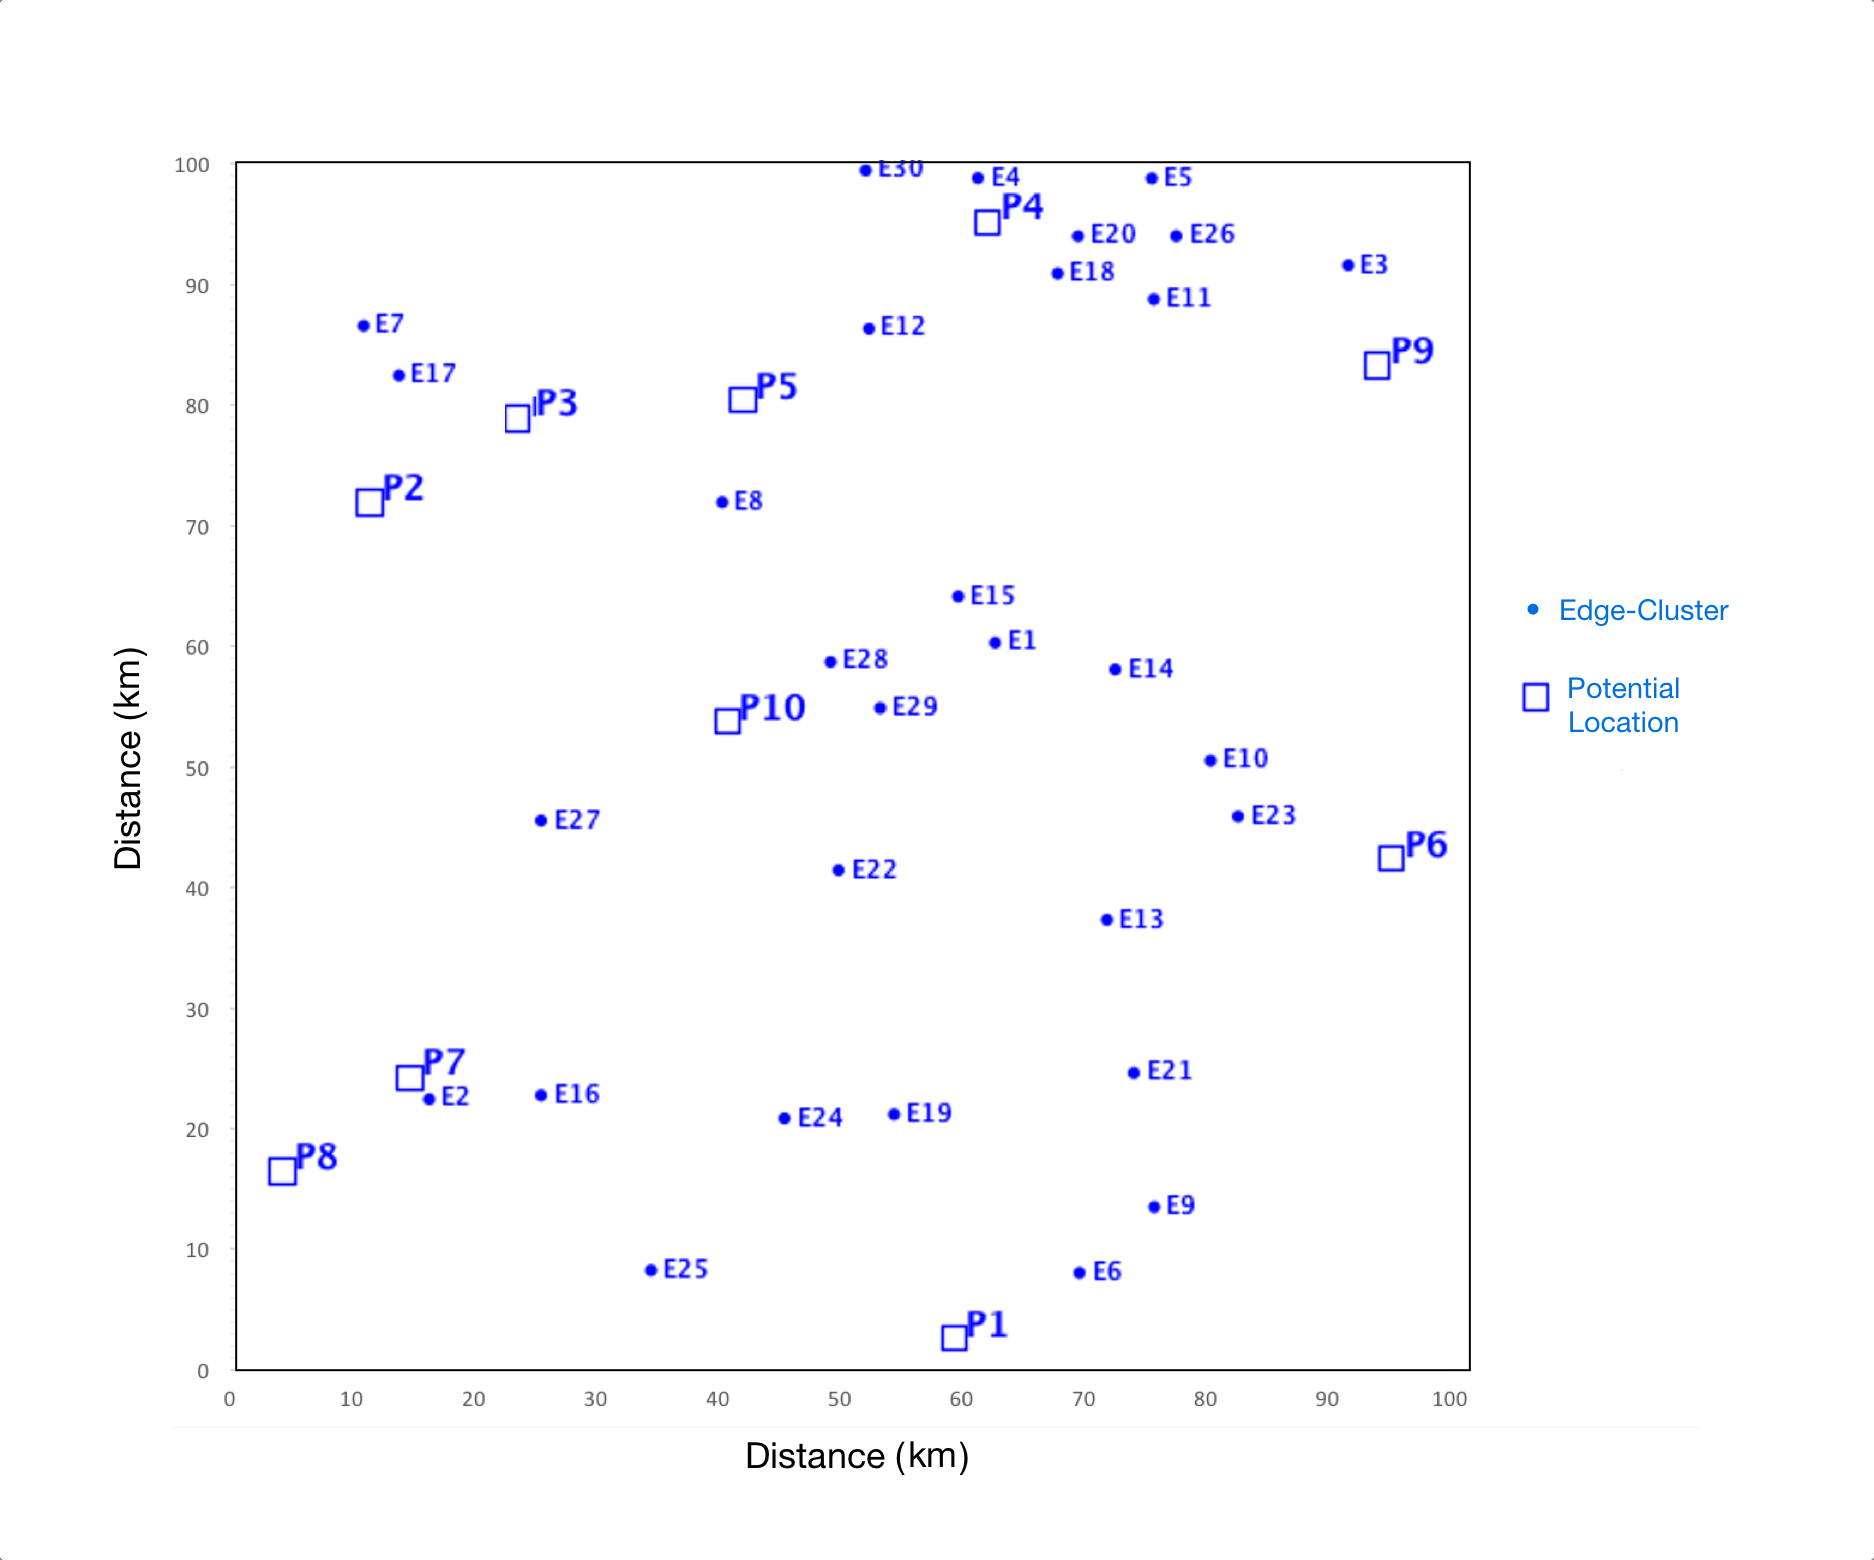
\includegraphics[trim=0 50 0 50,clip,width=3.8in]{100x100problem.png}}
%\caption{Edge-cluster locations and potential locations of fog for FPP3010 (instance-1)} 
%\label{nettopology}
%\end{figure}

%\subsubsection{Results from the Weighted Sum Method}
%Applied CPLEX to solve the FPP3010 (instance-1), we can find 7 solution frontiers (as shown by the 7 different solutions from Table~\ref{CPLEXresultssample}, the duplicated results are grey colored). The first column shows the solution index which makes reference to the 11 different weight combinations. The following two columns contain the decision output for the link type and the fog type at each location. Columns~4 and~5 provide the results of the two objective functions (cost and delay respectively) obtained with the weighted sum method. Finally, column 6 shows the relative Mixed-Integer Programming (MIP) gap. The MIP gap represents the percentage gap between the solution value found by CPLEX and the value of the optimal. For example, a 0.05 relative MIP gap means that CPLEX has found a solution that is five percent from the optimal. 
%%COMMENT: Here you talk about the 11 different weigth combinations...is this described somewhere in the paper? Maybe add a line or 2 when you present the weithted sum method (Section 4.1)?
%
%\begin{table}[tb]
%\centering
%\caption{CPLEX's result for problem FPP3010}
%\label{CPLEXresultssample}
%
%\resizebox{\columnwidth}{!}{
%\begin{tabular}{|c|c|c|c|c|c|}
%\hline
%\textbf{Solution} &\textbf{Link output}&\textbf{Fog output}&\textbf{Cost }&\textbf{Delay}  &\textbf{Gap}\\
%\textbf{number} &&&\textbf{(\$)}&\textbf{(ms)}& \textbf{(\%)}\\
%\hline
%\hline
%1&1 1 1 1 1 1 1 1 1 1	&4 1 4 3 4 4 4 4 4 4	&2586500.0&283&0.0\\
%2&1 1 1 1 1 1 1 0 1 1	&4 1 4 4 4 4 4 0 4 4	& \cellcolor{gray25}2078225.0& \cellcolor{gray25}283&9.94e-5\\
%3&1 1 1 1 1 1 1 0 1 1	&4 1 4 4 4 4 4 0 4 4	& \cellcolor{gray25}2078225.0& \cellcolor{gray25}283&9.98e-5\\
%4 &1 1 1 1 1 1 1 0 1 1	&4 1 4 4 4 4 4 0 4 4	&\cellcolor{gray25}2078225.0& \cellcolor{gray25}283&9.99e-5\\
%5&0 0 1 1 1 0 1 0 1 1	&0 0 4 4 4 0 4 0 4 4	&1507350.0&300&0.0047\\
%6&0 0 1 1 1 0 0 0 0 1	&0 0 4 4 4 0 0 0 0 4	&1004900.0&322&9.80e-5\\
%7&0 0 1 0 0 0 0 0 0 1	&0 0 4 0 0 0 0 0 0 4	&502450.0&356&7.69e-5\\
%8& 0 0 1 0 0 0 0 0 0 0	&0 0 4 0 0 0 0 0 0 0	&\cellcolor{gray25}251225.0& \cellcolor{gray25}384&0.0\\
%9& 0 0 1 0 0 0 0 0 0 0	&0 0 4 0 0 0 0 0 0 0	&\cellcolor{gray25}251225.0& \cellcolor{gray25}384&0.0\\
%10&0 0 0 0 0 0 0 0 0 0	&0 0 0 0 0 0 0 0 0 0	& \cellcolor{gray25}0.0& \cellcolor{gray25}449&0.0\\
%11&0 0 0 0 0 0 0 0 0 0	&0 0 0 0 0 0 0 0 0 0	& \cellcolor{gray25}0.0& \cellcolor{gray25}449&0.0\\
%\hline
%\end{tabular}}
%\end{table}
%
%Noticeably, different weight settings may converge to the same objective function values (for example, see solutions 2, 3, 4 from Table~\ref{CPLEXresultssample}). \Fig{CPLEXfro} plots the solution frontier obtained from the weighted sum method. 
%
%
%\subsubsection{Results from Evolutionary Algorithms}
%One fundamental difference between single and multiple objective optimization is the number of the solutions. Since several solutions can be optimal, each of these solutions represents a planning and routing scheme which considers a different cost/performance balance. An example of the 49 planning results (Pareto front) obtained with NSGA-II is presented in Table~\ref{table:solution.obj.nsgaii}. 
% 
\begin{figure*}[!t]
 	\subfloat[Solution frontier of weighted sum (CPLEX)]
       {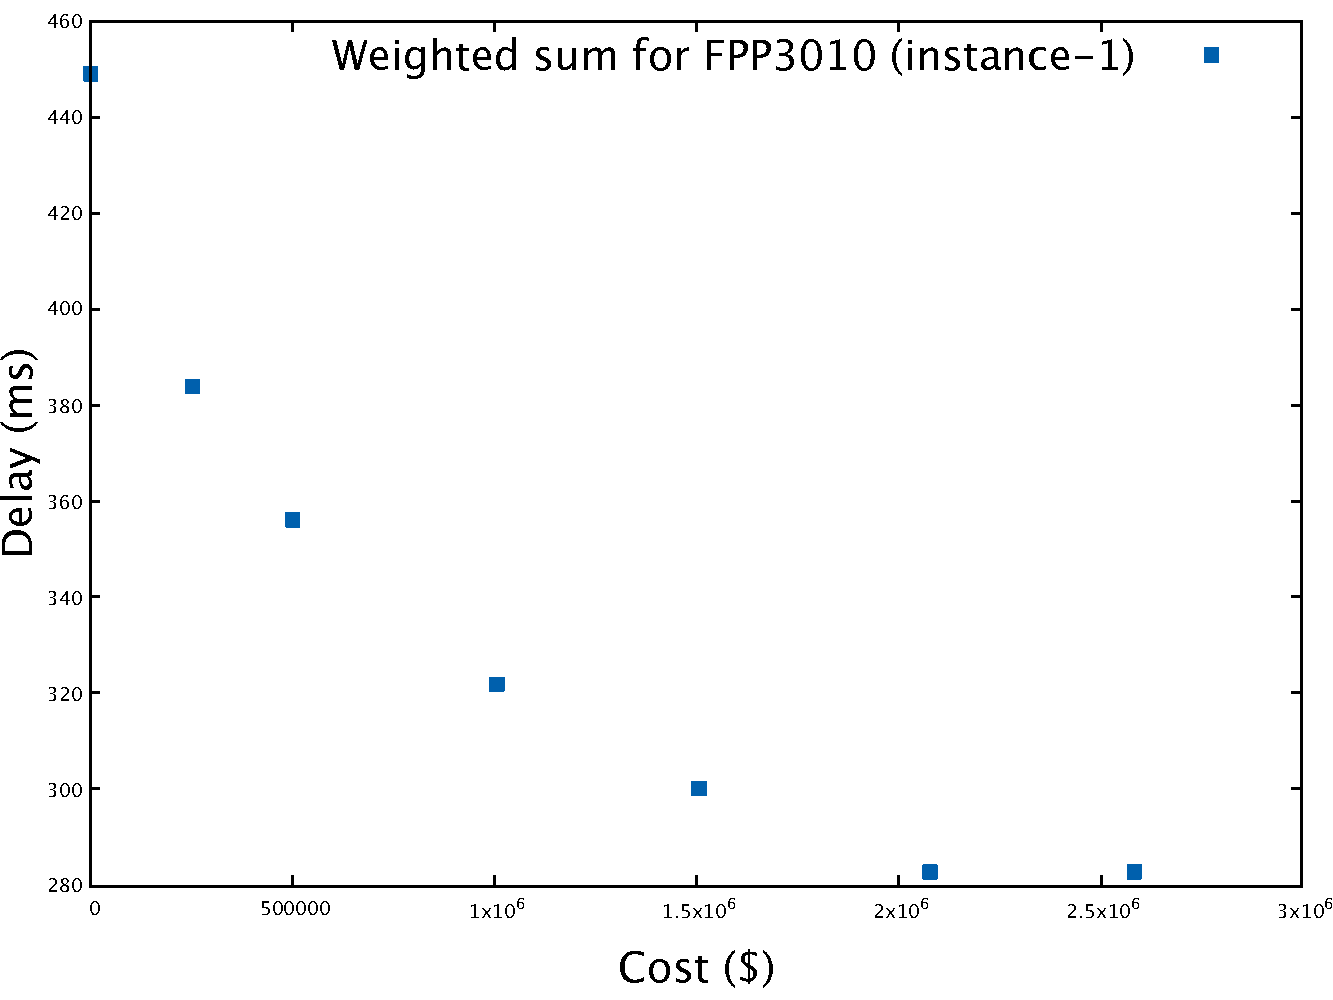
\includegraphics[trim=0 0 0 0,clip,width=0.5\linewidth]{ws_frontier.pdf}\label{CPLEXfro}} % first figure itself
       \hfil
        \subfloat[Solution frontier of NSGA-II]
        {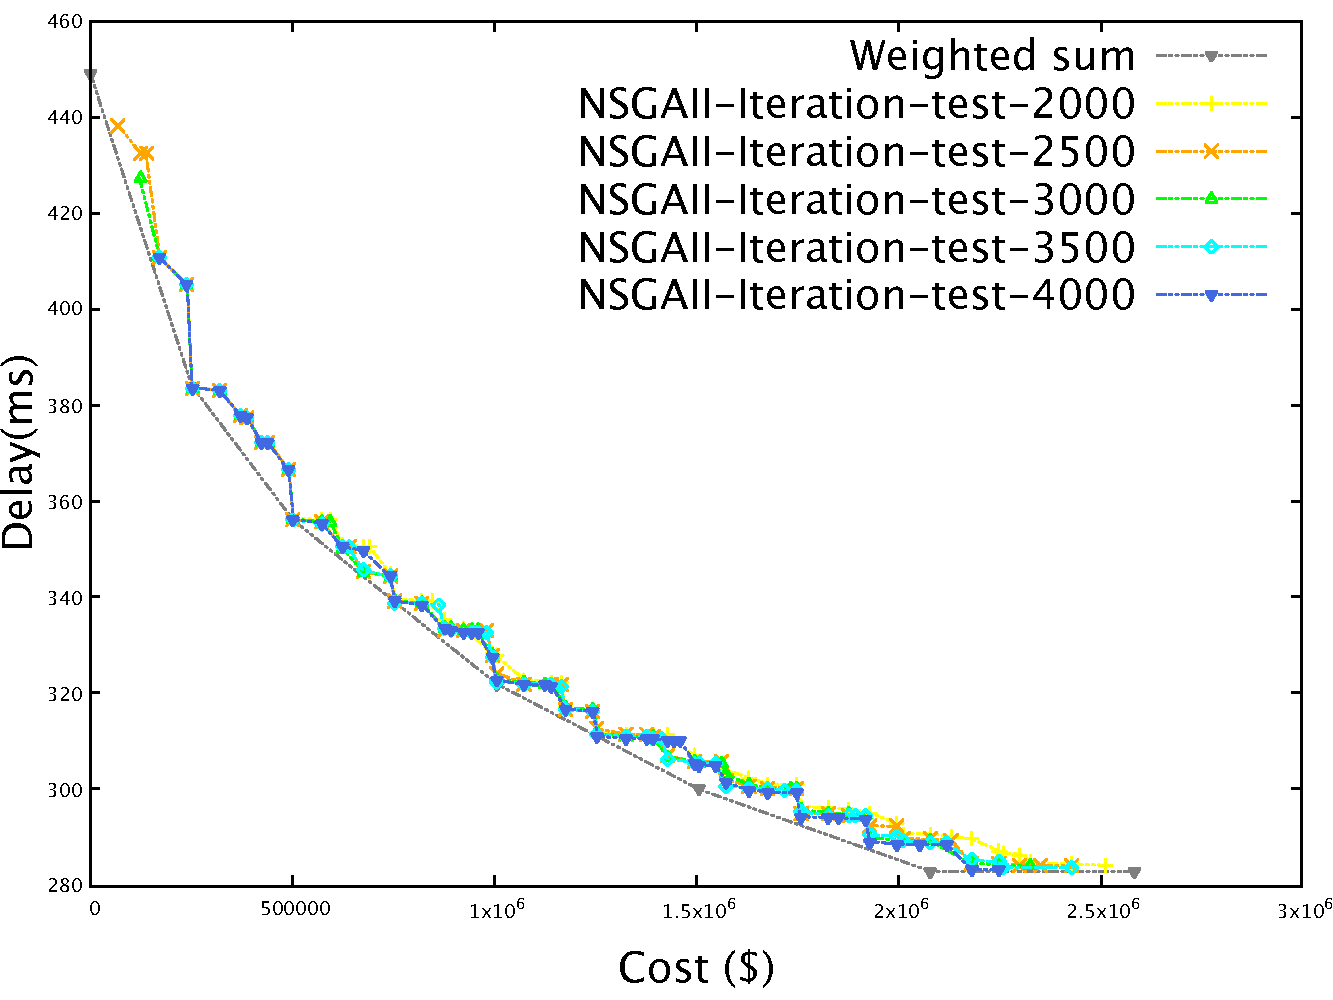
\includegraphics[trim =0 0 0 0,clip,width=0.5\linewidth]{nsga_frontier.pdf}\label{nsgafro}}% second figure itself
         %\captionsetup{font={scriptsize,}}
        
     % \vspace{10ex}

         
        % first figure itself
        % \captionsetup{font={scriptsize,}}
        \subfloat[Solution frontier of SMPSO]
        {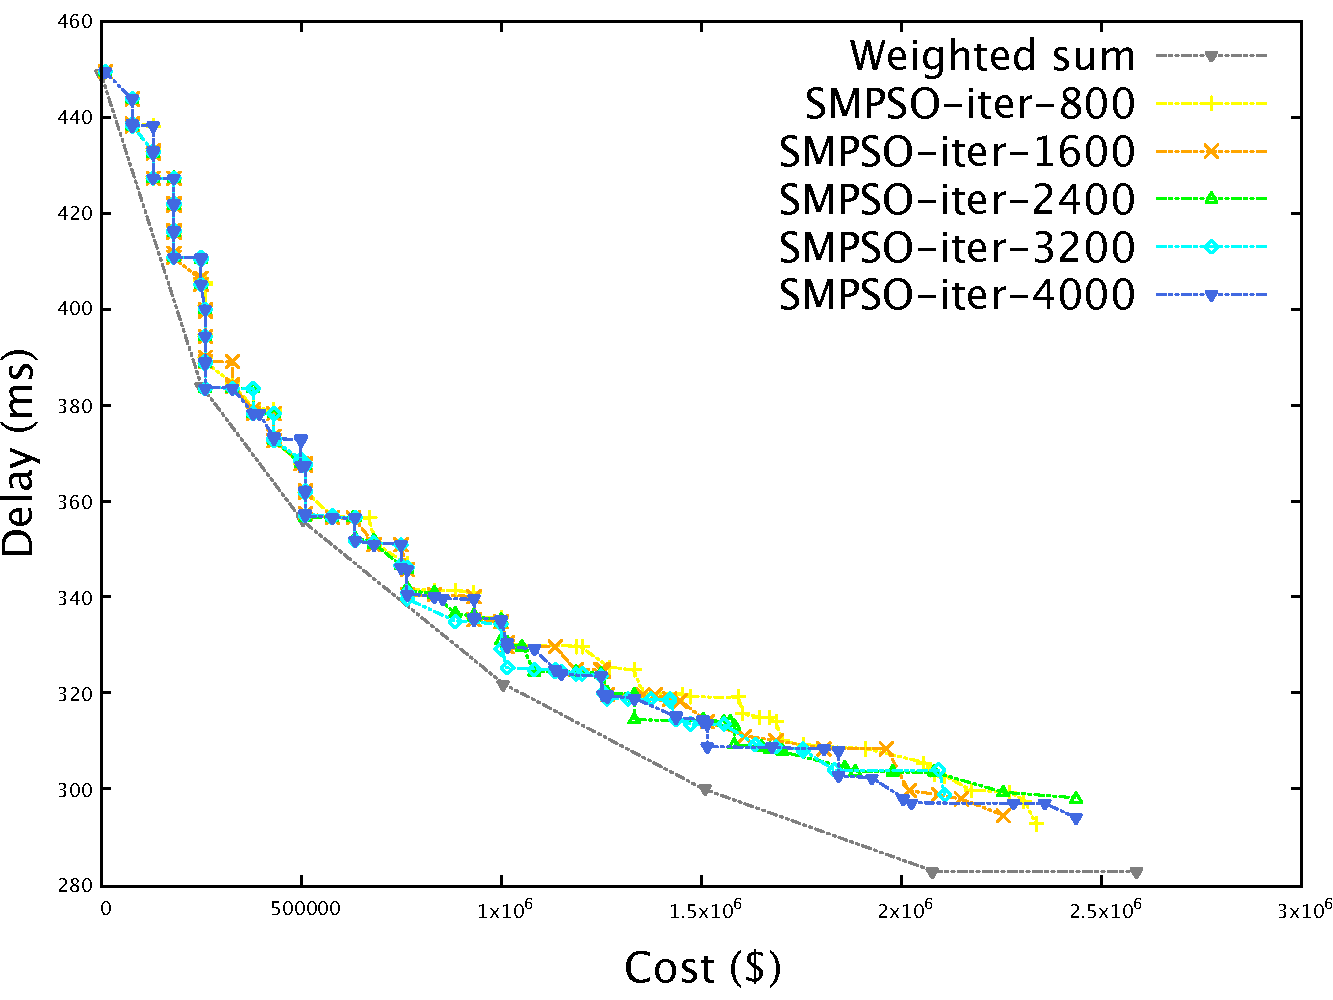
\includegraphics[trim=0 0 0 0,clip,width=0.5\linewidth]{smpso_frontier.pdf} \label{smpsofro}}
   \hfil
         % second figure itself
       % \captionsetup{font={scriptsize,}}
        \subfloat[Solution frontier of PSONSGA] 
        {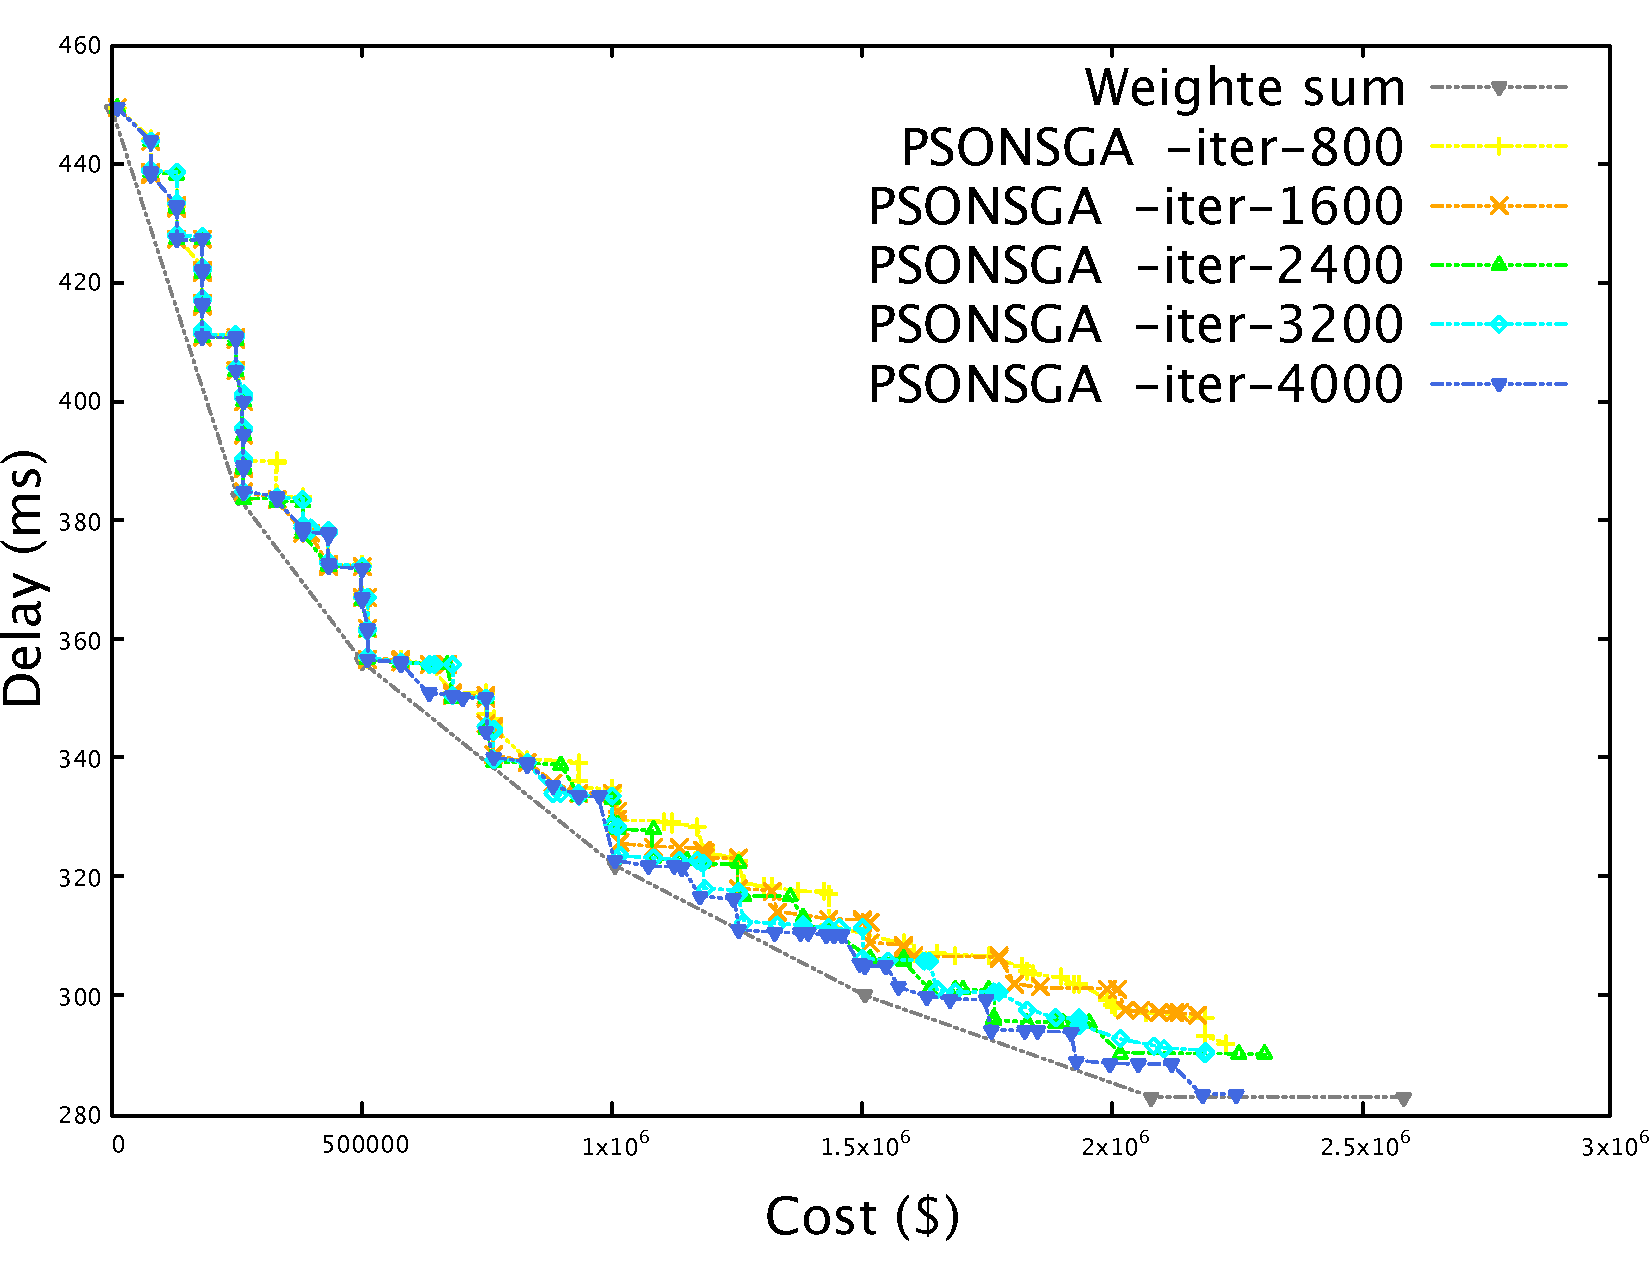
\includegraphics[trim=0 0 0 0,clip,width=0.5\linewidth]{psonsga_frontier2.pdf}\label{psonsgafro}}
\caption{Solution frontier comparison}
\end{figure*}

\begin{figure*}[!t]
    
        % first figure itself
     %   \captionsetup{font={scriptsize,}}
        \subfloat[Planning result of weighted sum (CPLEX), cost: \$1,004,900 delay: 322.1ms]
        {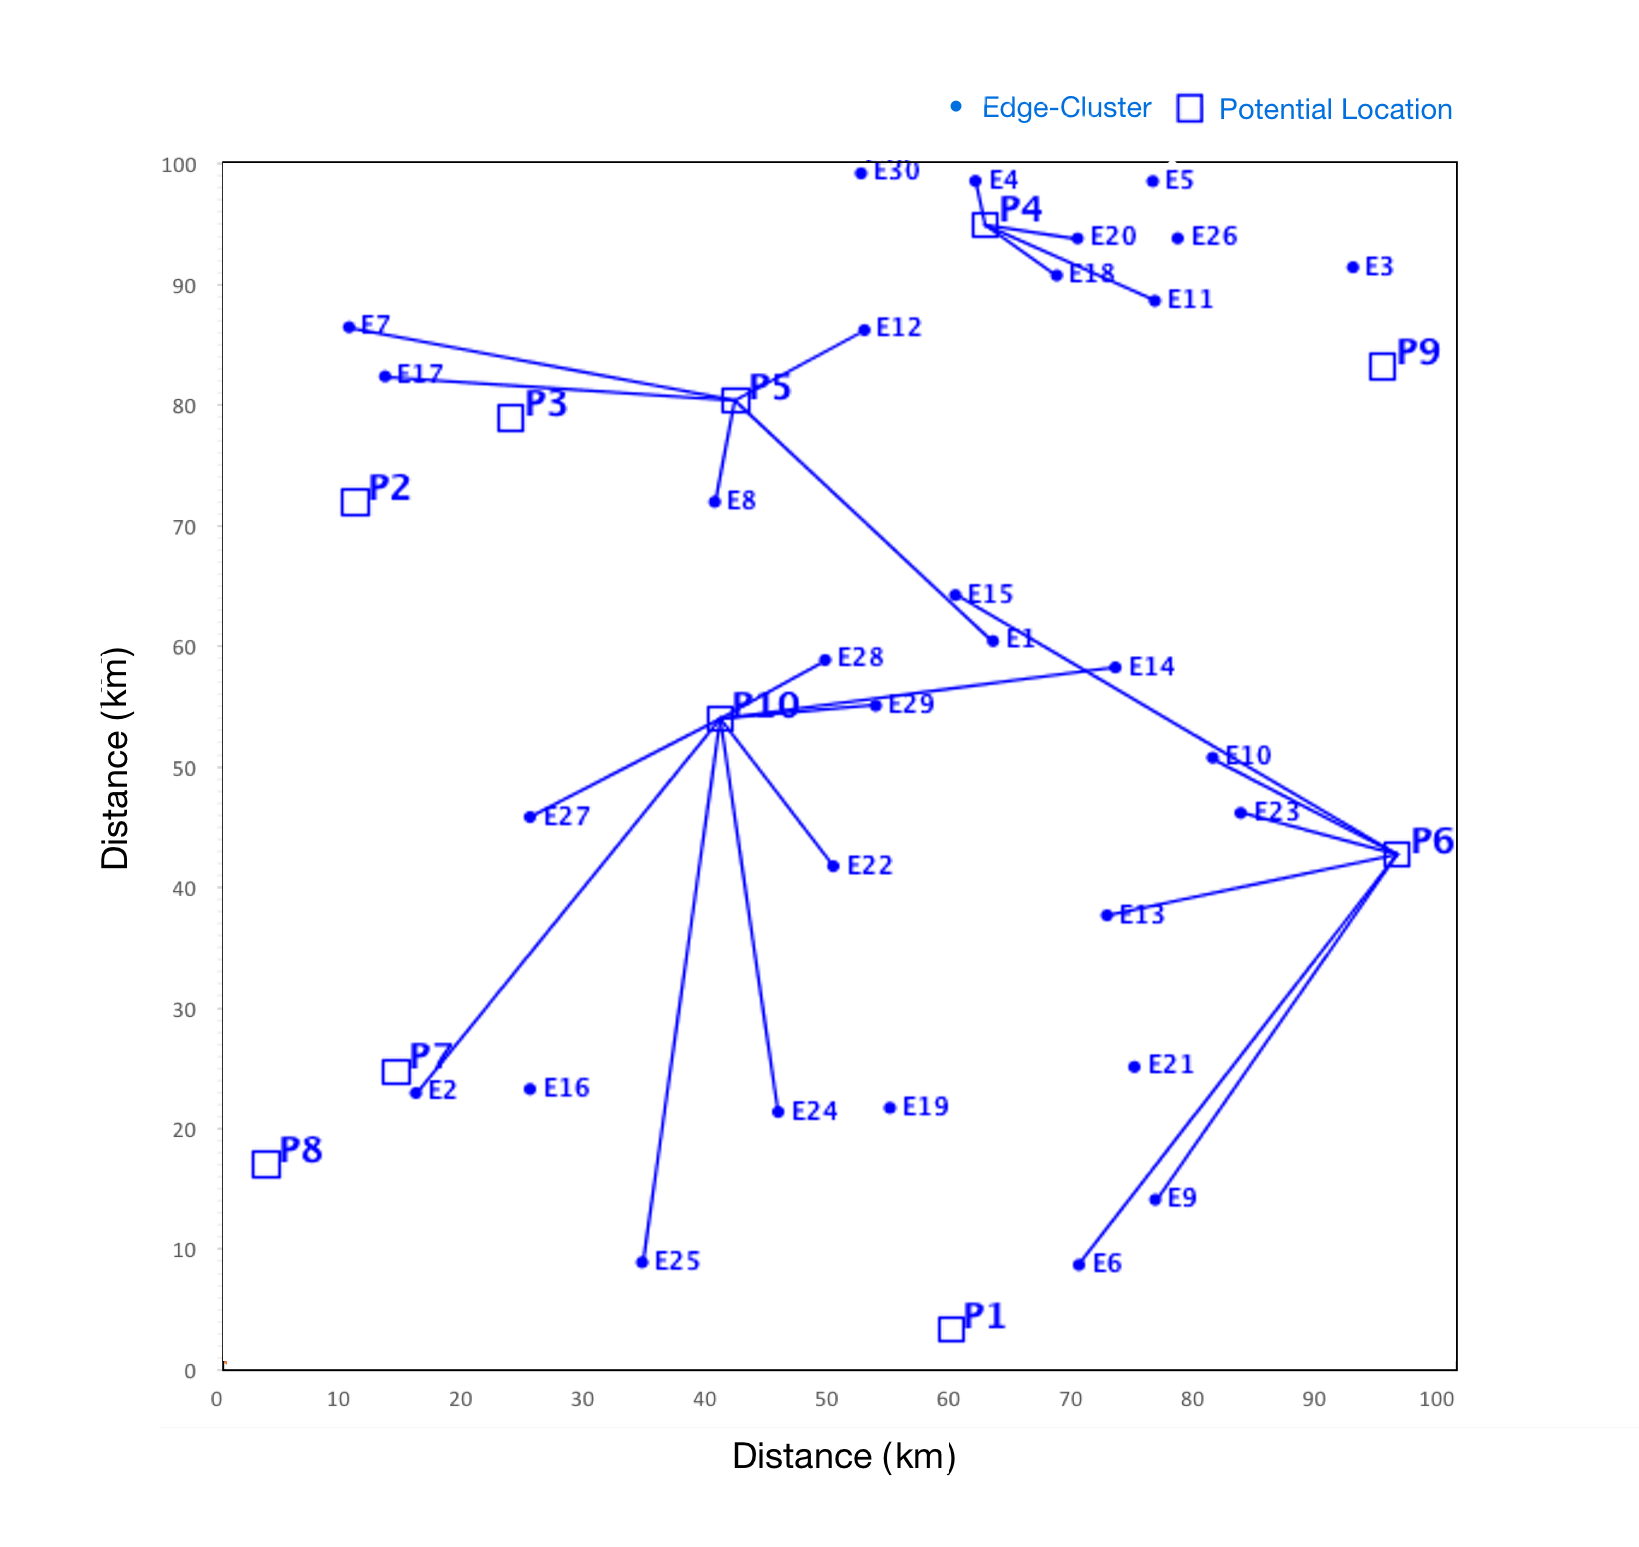
\includegraphics[trim=40 20 20 30,clip,width=.5\linewidth]{100x100problem_cplex2.png}\label{CPLEXrouting}}
    \hfil
        % second figure itself
       %  \captionsetup{font={scriptsize,}}
        \subfloat[Planning result of NSGA-II, cost: \$1,004,900 delay: 322.6ms]
        {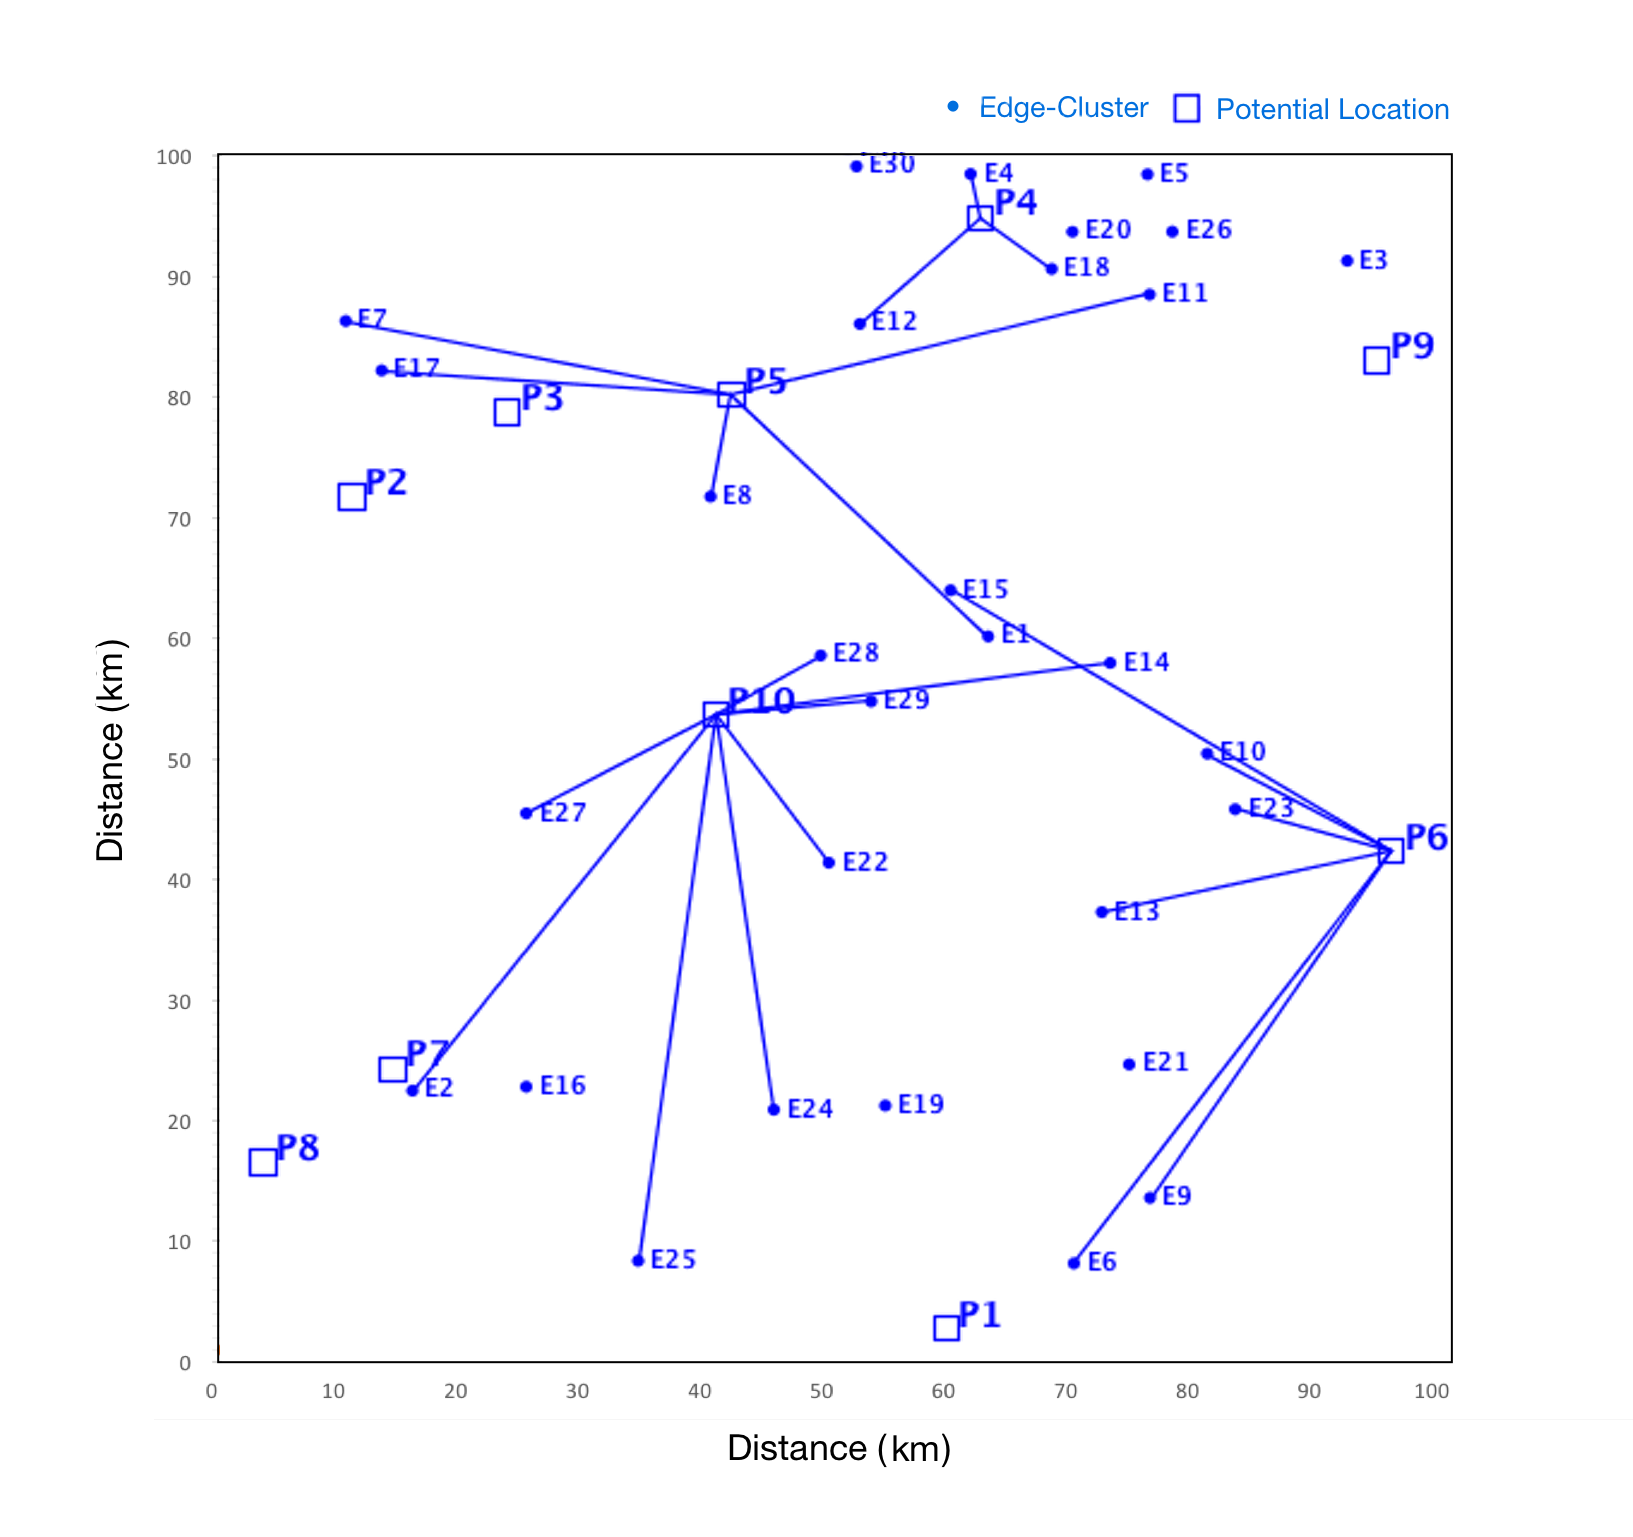
\includegraphics[trim =40 20 20 40,clip,width=0.5\linewidth]{100x100problem_nsga2.png}\label{nsgarouting}}
  
   \end{figure*}
   \begin{figure*}[!t]   % first figure itself
         %\captionsetup{font={scriptsize,}}
        \subfloat[Planning result of SMPSO, cost: \$1,004,900 delay: 323.8ms]
        { 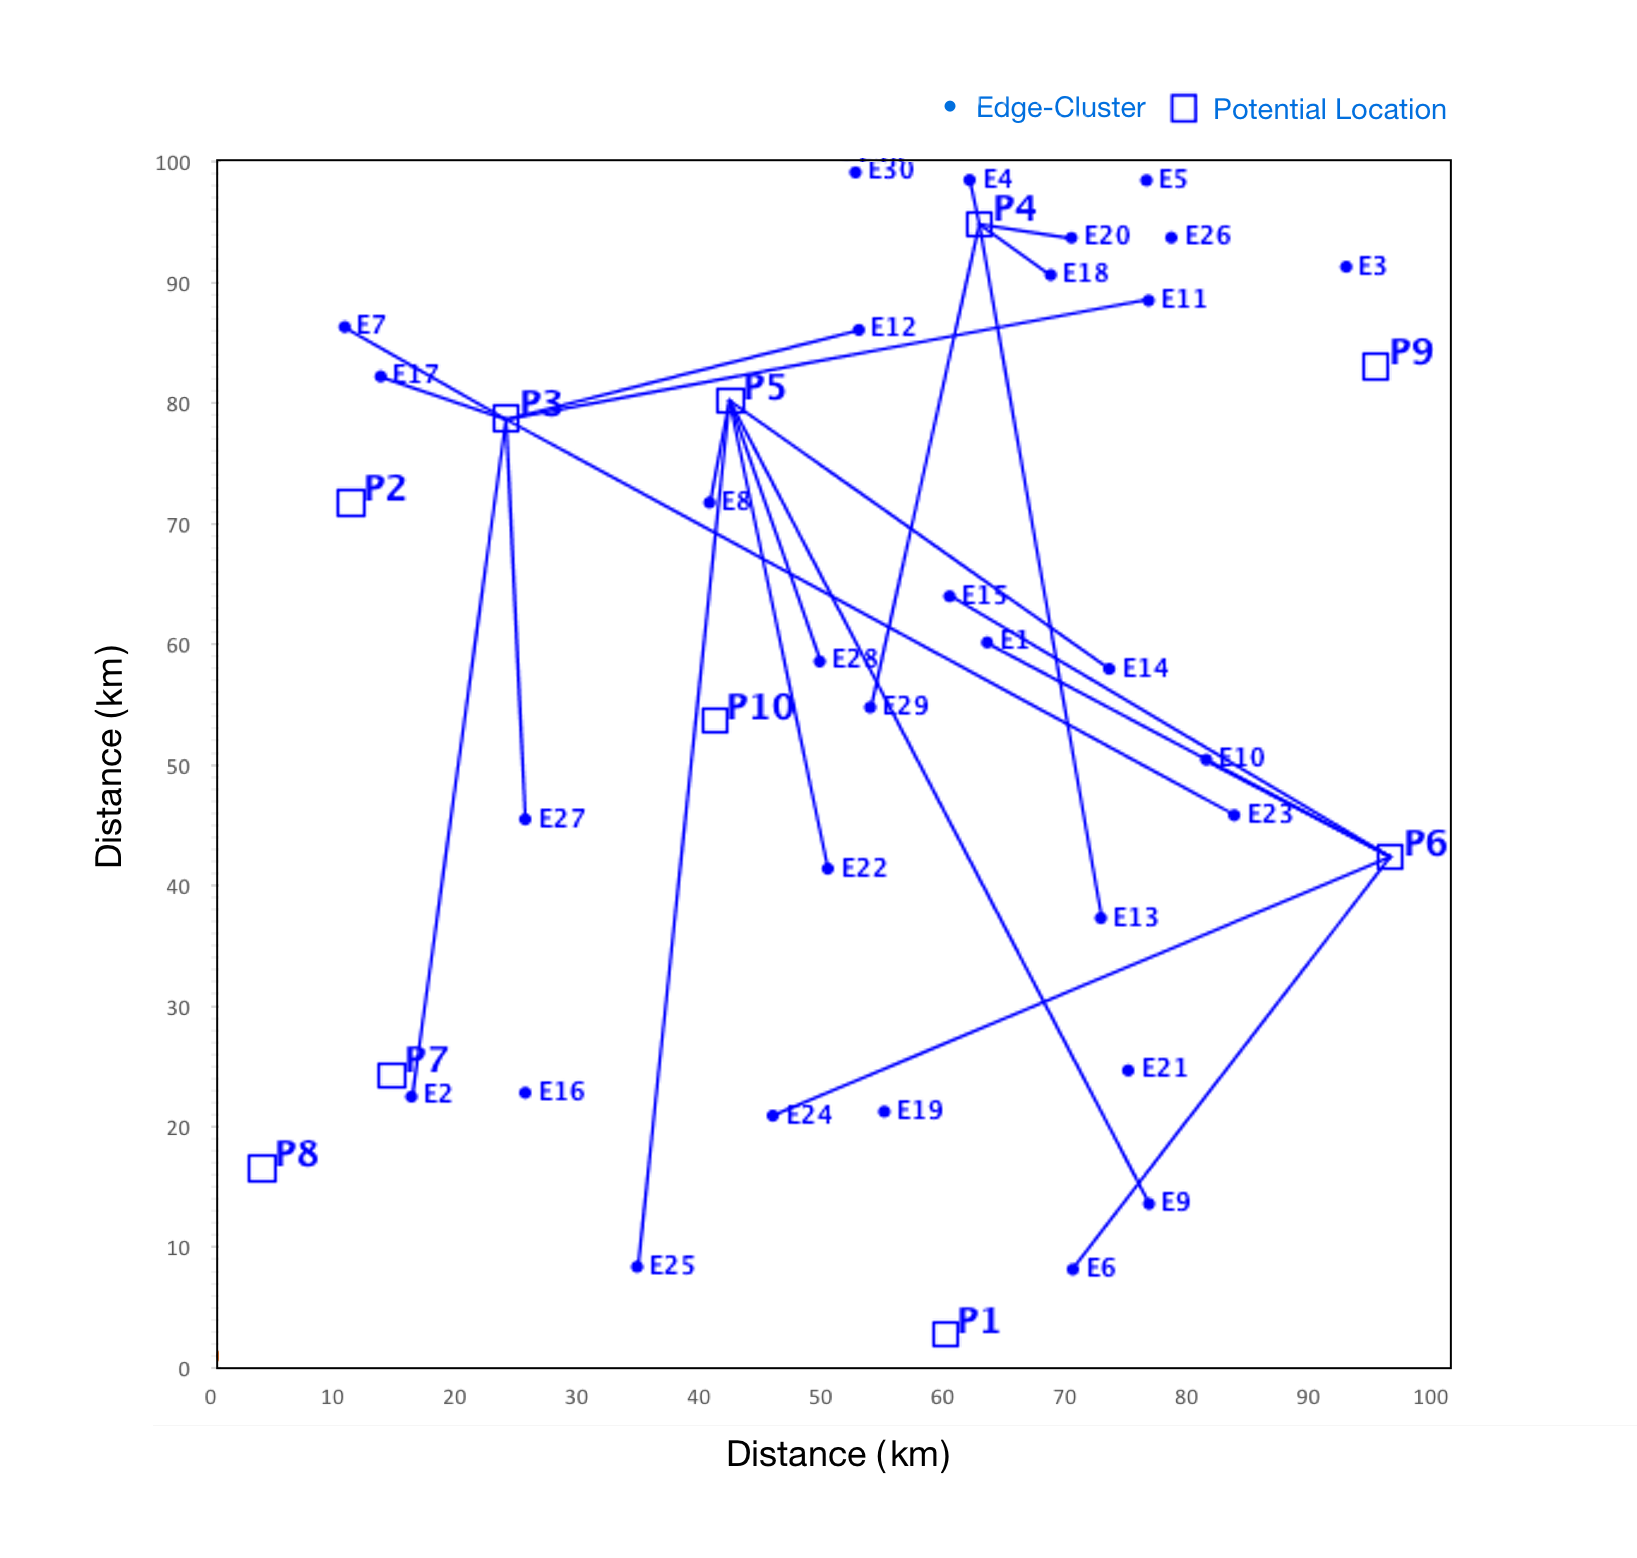
\includegraphics[trim=40 26 20 40,clip,width=.5\linewidth]{100x100problem_smpso2.png} \label{smpsorouting}}
\hfil
       % second figure itself
     %   \captionsetup{font={scriptsize,}}
        \subfloat[Planning result of PSONSGA, cost: \$1,004,900 delay: 322.7ms]
        {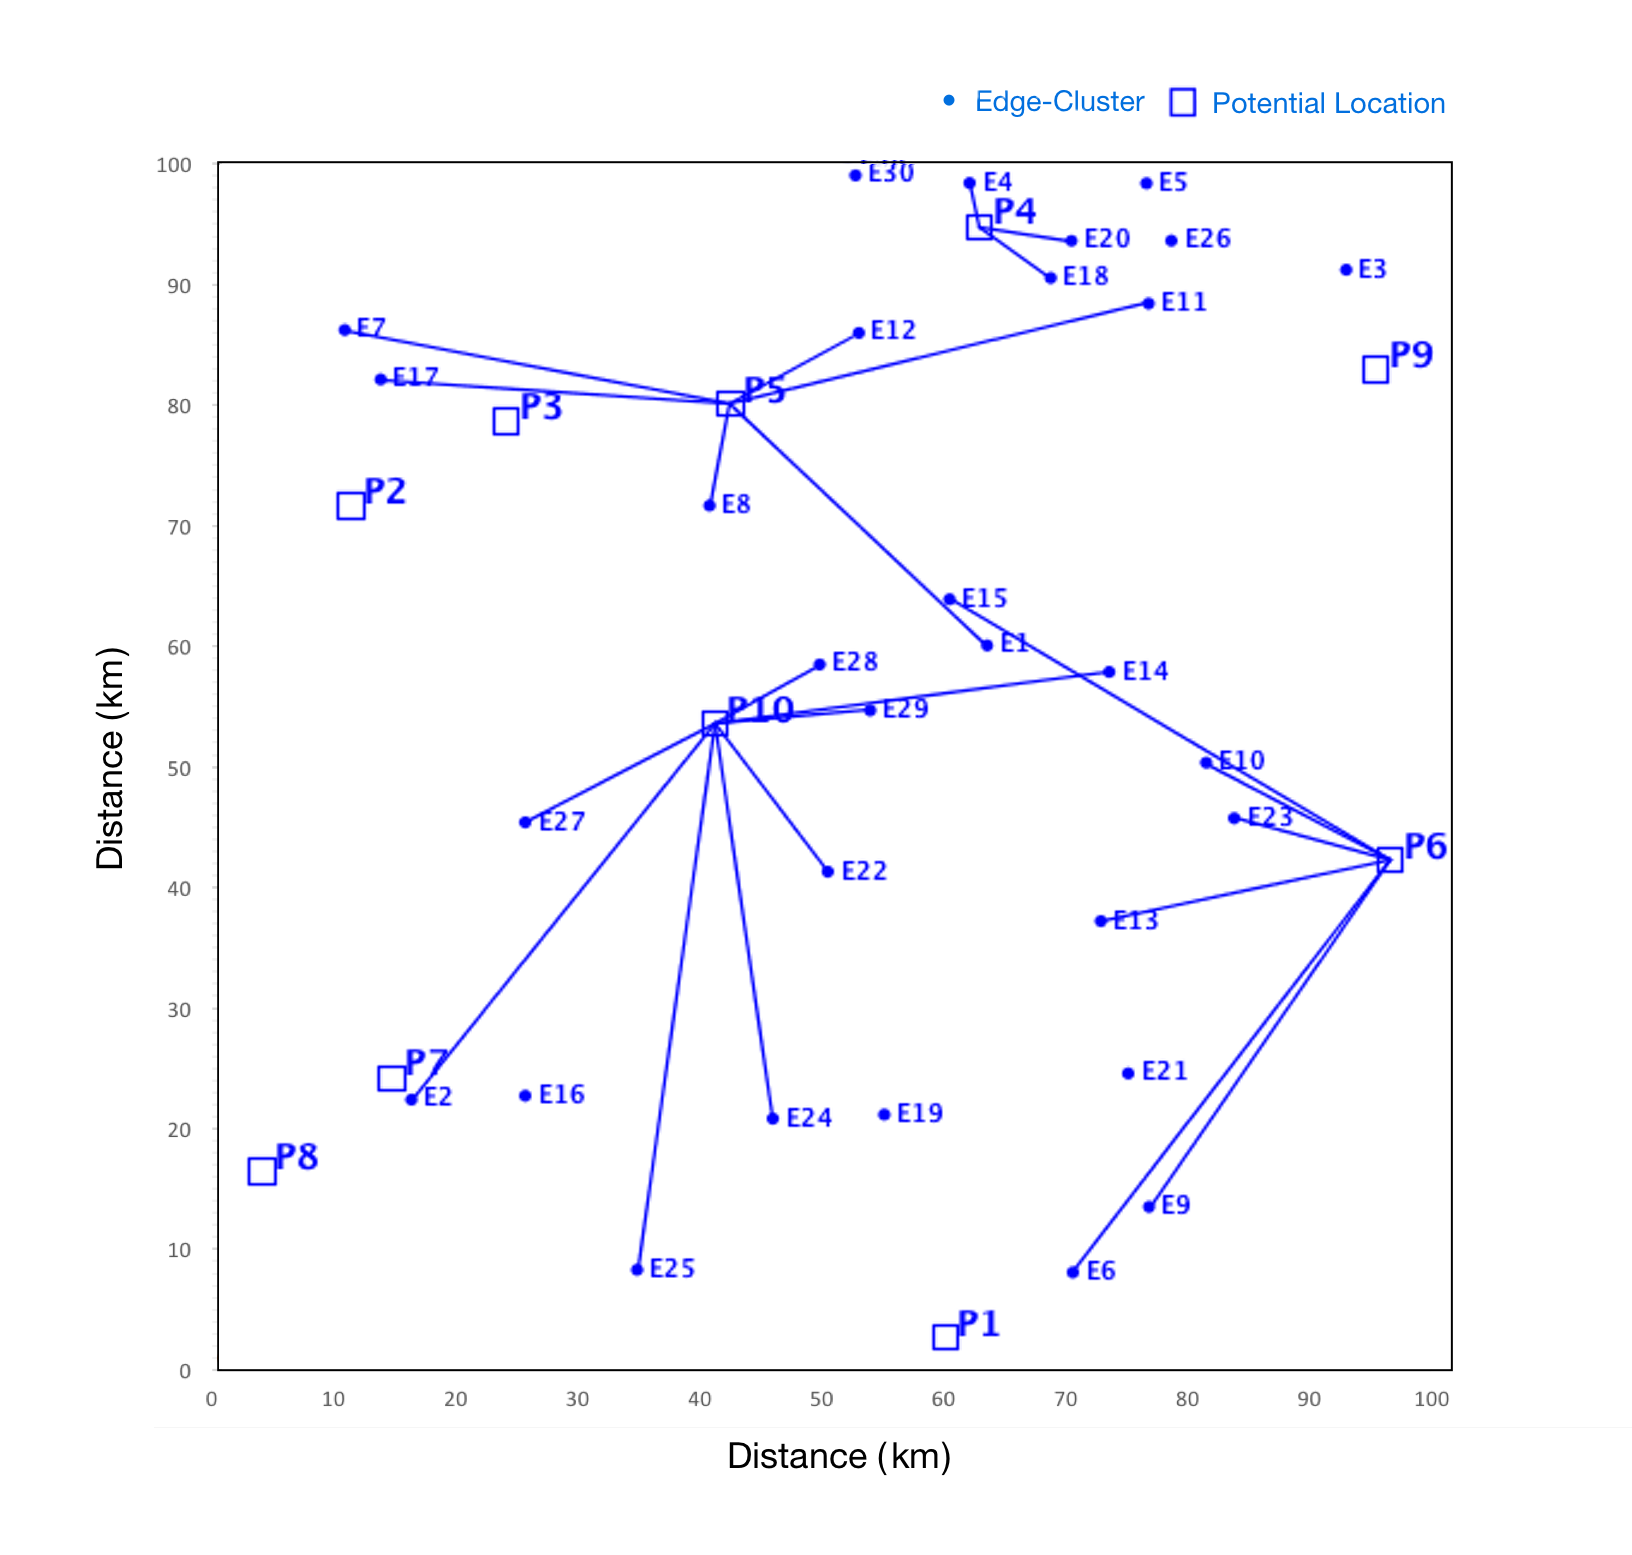
\includegraphics[trim=40 26 20 30,clip,width=.5\linewidth]{100x100problem_psonsga2.png}\label{psonsgarouting}}
    \caption{Planning result comparison}
\end{figure*}
%
%
%The first column shows the solution number. The following two columns contain the cost and delay results obtained by the NSGA-II algorithm. Columns~4 and~5 provide, respectively, the decision variables for the link and fog type at each location, where ``0" indicates that no facility is installed, and subsequent numbers correspond to different facility types (fog or link). The following two columns show the CPLEX's results (cost and delay values). Since CPLEX only produces 7 solution frontiers, the non-existing solution rows are labelled as ``NA". Finally, the cost gaps and delay gaps between solutions from the NSGA-II and corresponding solution from the weighted sum is provided in the last two columns. 
%The solution frontiers, for FPP3010 by applying NSGA-II, SMPSO, PSONSGA, are plotted in Figures \ref{nsgafro}, \ref{smpsofro} and \ref{psonsgafro}.
%%COMMENT: Do you need to represent the COPLEX results since they are already presented in a previous table? Maybe you could remove columns 6 and 7?
%
%\begin{table}[ht]
%\caption{NSGA-II's solution set for FPP3010 (instance-1)}\label{table:solution.obj.nsgaii}
%\centering
%\resizebox{\columnwidth}{!}{
%\tiny
%\begin{tabular}{|*{9}{r|}}
%\hline
% &\multicolumn{4}{|c|}{\textbf{NSGA-II}} &\multicolumn{2}{c|}{\textbf{Weighted Sum}} &&\\
% \hline
%\textbf{Solution }&	\textbf{Cost }	&\textbf{Delay 	}	&\textbf{Variables-link}&\textbf{Variables-fog}&\textbf{Cost }	&\textbf{Delay }	&\textbf{Cost diff}	&\textbf{Delay diff}\\
%\textbf{num}&	\textbf{ (\$)}	&\textbf{(ms)	}	&&&\textbf{(\$)}	&\textbf{ (ms)}	&\textbf{(\%) }	&\textbf{(\%)}\\
%
%\hline
%
%1	&121225	&   427.2	&0 0 0 0 0 0 0 0 0 1	&0 0 0 0 0 0 0 0 0 2	&			NA	&NA&&\\
%2	&171225	&   410.8	&0 0 1 0 0 0 0 0 0 0	&0 0 3 0 0 0 0 0 0 0	&			NA	&NA&&\\
%3	&239650	&   405.0	&1 0 1 0 0 0 0 0 0 0	&1 0 3 0 0 0 0 0 0 0	&			NA	&NA&&\\
%4	&251225	&   383.7	&0 0 1 0 0 0 0 0 0 0	&0 0 4 0 0 0 0 0 0 0	&	      \cellcolor{blizzardblue} 251225&	\cellcolor{blizzardblue}383.7	&\cellcolor{blizzardblue}0	&\cellcolor{blizzardblue}0.00\%\\
%5	&319650	&   383.1	&0 0 1 0 0 0 0 0 1 0	&0 0 4 0 0 0 0 0 1 0	&			NA	&NA&&\\
%6	&372450	&   377.8	&0 0 1 0 0 0 0 0 1 0	&0 0 4 0 0 0 0 0 2 0	&			NA	&NA&&\\
%7	&388075	&   377.6	&0 1 0 0 0 1 1 0 0 0	&0 1 0 0 0 1 4 0 0 0	&			NA	&NA&&\\
%8	&422450	&   372.3	&0 0 1 0 0 0 0 0 0 1	&0 0 3 0 0 0 0 0 0 4	&			NA	&NA&&\\
%9	&440875	&   372.2	&0 0 1 0 1 0 0 0 0 1	&0 0 1 0 2 0 0 0 0 4	&			NA	&NA&&\\
%10	&490875	&   366.6	&1 0 1 0 0 0 0 0 0 1	&1 0 4 0 0 0 0 0 0 3	&			NA	&NA&&\\
%11	&502450	&   356.2	&0 0 1 0 0 0 0 0 0 1	&0 0 4 0 0 0 0 0 0 4	&	      \cellcolor{blizzardblue} 502450	&\cellcolor{blizzardblue}356.1	&\cellcolor{blizzardblue}0	&\cellcolor{blizzardblue}0.03\%\\
%12	&570875	&   355.5	&1 0 1 0 0 0 0 0 0 1	&1 0 4 0 0 0 0 0 0 4	&			NA	&NA&&\\
%13	&623675	&   350.4	&1 0 1 1 0 0 0 0 0 0	&2 0 4 4 0 0 0 0 0 0	&			NA	&NA&&\\
%14	&673675	&   350.0	&0 0 1 1 0 0 0 0 0 1	&0 0 3 4 0 0 0 0 0 4	&			NA	&NA&&\\
%15	&692100	&   350.0	&0 1 0 0 0 0 1 0 1 1	&0 1 0 0 0 0 4 0 2 4	&			NA	&NA&&\\
%16	&742100	&   344.5	&1 0 1 1 0 0 0 0 0 1	&1 0 4 3 0 0 0 0 0 4	&			NA	&NA&&\\
%17	&753675	&   339.3	&0 0 1 1 0 0 0 0 0 1	&0 0 4 4 0 0 0 0 0 4	&			NA	&NA&&\\
%18	&822100	&   338.8	&1 0 1 1 0 0 0 0 0 1	&1 0 4 4 0 0 0 0 0 4	&			NA	&NA&&\\
%19	&874900	&   333.6	&1 0 1 1 0 0 0 0 0 1	&2 0 4 4 0 0 0 0 0 4	&			NA	&NA&&\\
%20	&890525	&   333.4	&1 0 1 1 0 0 1 0 0 1	&1 0 4 4 0 0 1 0 0 4	&			NA	&NA&&\\
%21	&924900	&   333.2	&0 0 1 1 1 0 0 0 0 1	&0 0 4 4 3 0 0 0 0 4	&			NA	&NA&&\\
%22	&993325	&   327.6	&0 0 1 1 1 0 1 0 1 0	&0 0 3 4 4 0 4 0 1 0	&			NA	&NA&&\\
%23	&1004900&   322.6	&0 0 1 1 1 0 0 0 0 1	&0 0 4 4 4 0 0 0 0 4	&	\cellcolor{blizzardblue}       1004900	&\cellcolor{blizzardblue}322.1&\cellcolor{blizzardblue}	0	&\cellcolor{blizzardblue}0.17\%\\
%24	&1073325&   322.0	&0 0 1 1 1 0 1 0 1 0	&0 0 4 4 4 0 4 0 1 0	&			NA	&NA&&\\
%25	&1141750&   321.8	&1 1 0 1 0 1 1 0 0 1	&1 1 0 4 0 4 4 0 0 4	&			NA	&NA&&\\
%26	&1176125&   317.1	&0 0 1 1 1 0 1 0 1 0	&0 0 4 4 4 0 4 0 3 0	&			NA	&NA&&\\
%27	&1244550&   316.4	&1 0 1 1 1 0 1 0 1 0	&3 0 1 4 4 0 4 0 4 0	&			NA	&NA&&\\
%28	&1256125&   311.5	&0 0 1 1 0 0 1 0 1 1	&0 0 4 4 0 0 4 0 4 4	&			NA	&NA&&\\
%29	&1324550&   311.3	&1 1 0 1 0 1 1 0 0 1	&1 4 0 4 0 4 4 0 0 4	&			NA	&NA&&\\
%30	&1377350&   311.2	&1 0 0 1 1 1 1 0 1 0	&2 0 0 4 4 4 4 0 4 0	&			NA	&NA&&\\
%31	&1392975&   311.0	&1 1 0 1 1 1 1 0 0 1	&1 4 0 4 1 4 4 0 0 4	&			NA	&NA&&\\
%32	&1415775&   311.0	&0 1 0 1 1 1 1 1 0 1	&0 4 0 4 3 4 3 1 0 4	&			NA	&NA&&\\
%33	&1445775&   310.9	&1 0 1 1 1 1 1 0 1 0	&2 0 1 4 4 4 4 0 4 0	&			NA	&NA&&\\
%34	&1495775&   306.1	&1 0 1 1 1 1 1 0 1 0	&3 0 1 4 4 4 4 0 4 0	&			NA	&NA&&\\
%35	&1507350&   305.6	&0 0 1 1 1 0 1 0 1 1	&0 0 4 4 4 0 4 0 4 4	&	  \cellcolor{blizzardblue}     1507350	&\cellcolor{blizzardblue}299.9	&\cellcolor{blizzardblue}0	&\cellcolor{blizzardblue}1.87\%\\
%36	&1575775&   301.3	&1 0 1 1 1 0 1 0 1 1	&1 0 4 4 4 0 4 0 4 4	&			NA	&NA&&\\
%37	&1628575&   300.6	&1 0 1 1 0 1 1 0 1 1	&4 0 4 4 0 2 4 0 4 4	&			NA	&NA&&\\
%38	&1678575&   300.2	&1 0 1 1 1 0 1 0 1 1	&3 0 4 4 4 0 4 0 4 4	&			NA	&NA&&\\
%39	&1697000&   300.1	&1 1 0 1 1 1 1 0 1 1	&4 4 0 4 4 4 1 0 4 2	&			NA	&NA&&\\
%40	&1747000&   299.9	&1 1 0 1 1 1 1 0 1 1	&4 4 0 4 4 4 1 0 4 3	&			NA	&NA&&\\
%41	&1758575&   295.1	&1 0 1 1 1 0 1 0 1 1	&4 0 4 4 4 0 4 0 4 4	&			NA	&NA&&\\
%42	&1827000&   294.6	&1 0 1 1 1 1 1 0 1 1	&4 0 4 4 4 1 4 0 4 4	&			NA	&NA&&\\
%43	&1929800&   292.0	&1 0 1 1 1 1 1 0 1 1	&4 0 4 4 3 4 4 0 4 4	&			NA	&NA&&\\
%44	&1998225&   289.8	&1 1 1 1 1 1 1 0 1 1	&4 1 4 4 4 4 4 0 4 3	&			NA	&NA&&\\
%45	&2009800&   289.2	&1 0 1 1 1 1 1 0 1 1	&4 0 4 4 4 4 4 0 4 4	&			NA	&NA&&\\
%46	&2078225&   289.0	&1 1 1 1 1 1 1 0 1 1	&4 1 4 4 4 4 4 0 4 4	&	     \cellcolor{blizzardblue}  2078225	&\cellcolor{blizzardblue}283.2	&\cellcolor{blizzardblue}0&\cellcolor{blizzardblue}	2.03\%\\
%47	&2181025&   284.5	&1 0 1 1 1 1 1 1 1 1	&4 0 4 3 4 4 4 4 4 4	&	      \cellcolor{blizzardblue} 2148225.151&	\cellcolor{blizzardblue}282.8	&\cellcolor{blizzardblue}-0.015038731	&\cellcolor{blizzardblue}0.60\%\\
%48	&2249450&   284.4	&1 1 1 1 1 1 1 1 1 1	&4 1 4 3 4 4 4 4 4 4	&	      \cellcolor{blizzardblue} 2586500	&\cellcolor{blizzardblue}282.7	&\cellcolor{blizzardblue}0.149836627	&\cellcolor{blizzardblue}0.61\%\\
%49	&2261025&   284.1	&1 0 1 1 1 1 1 1 1 1	&4 0 4 4 4 4 4 4 4 4	&			NA&	NA&&\\
%\hline
%\end{tabular}}
%\end{table}
%
The network design for one solution (cost: \$1,004,900, delay: 322.1ms) in approximate pareto front is plottd in \Fig{nsgarouting}. The counterpart from Weighted sum, SMPSO and PSONSGA with same cost are also plotted respectively, in Figures~\ref{CPLEXrouting},~\ref{smpsorouting} and~\ref{psonsgarouting}. The detailed examination shows that both NSGA and PSONSGA generate the same fog network setup (fog node placement, fog node selection, and link selection) as the exact algorithm (weighted sum). For the same capital expenditure, the results from Weighted sum, NSGA-II, SMPSO and PSONSGA give 322.1ms, 322.6ms, 323.8ms and 322.7ms delay respectively. The minor delay differences are due to the misplacement of a small number of edge-clusters (see E11 and E12 for example). These differences can be compensated through user-relocation and load-balancing schemes. This topic has been thoroughly researched in cloud computing, and mature research results can be applied on this relocation subproblem.


\subsection{Result Analysis}\label{resultanalyssi}
In this section, we present the expriment results to assess the performance of the algorithms.
%Four instances of 26 different problem sizes are solved by the weighted sum, NSGA-II, SMPSO and PSONSGA algorithms. %COMMENT: This line seems repetitive as you already mentioned this previously...remove?
A population size of 100 with a number of iterations of 10,000 is used for the three evolutionary algorithms. We use the same parameter settings as the ones described in the last section. %COMMENT: Why these values for the population size and the number of iterations? do they provide best results?


\subsubsection{HV Indicator Comparison}
Since the output of each MO algorithm is a non-dominated solution set, we employ the HV indicator~\cite{Auger:2009:THI:1527125.1527138} to evaluate and compare the solution quality between the weighted sum algorithm and the three evolutionary algorithms. 

The HV indicator examines both the convergence and diversity properties of a solution set. In these perspectives, PSONSGA algorithm displays its superiority in finding a good quality solution within reasonable computation time. In fact, for all four problem instances (a total of 104 different problems), PSONSGA provides the best HV value for 95 problems (91.3\%). The NSGA-II and SMPSO each provides the highest HV value for 19 different problems (18.2\%). The weighted sum approach only provides the best HV value for 2 problems (1.92\%).

\Fig{hvaverage} provides a complete comparison of the HV values amongst the weighted sum, NSGA-II, SMPSO and PSONSGA algorithms over the four instance sets with a 95\% confidence interval.
%%%REVISED
\begin{figure*}[ht]
\centerline{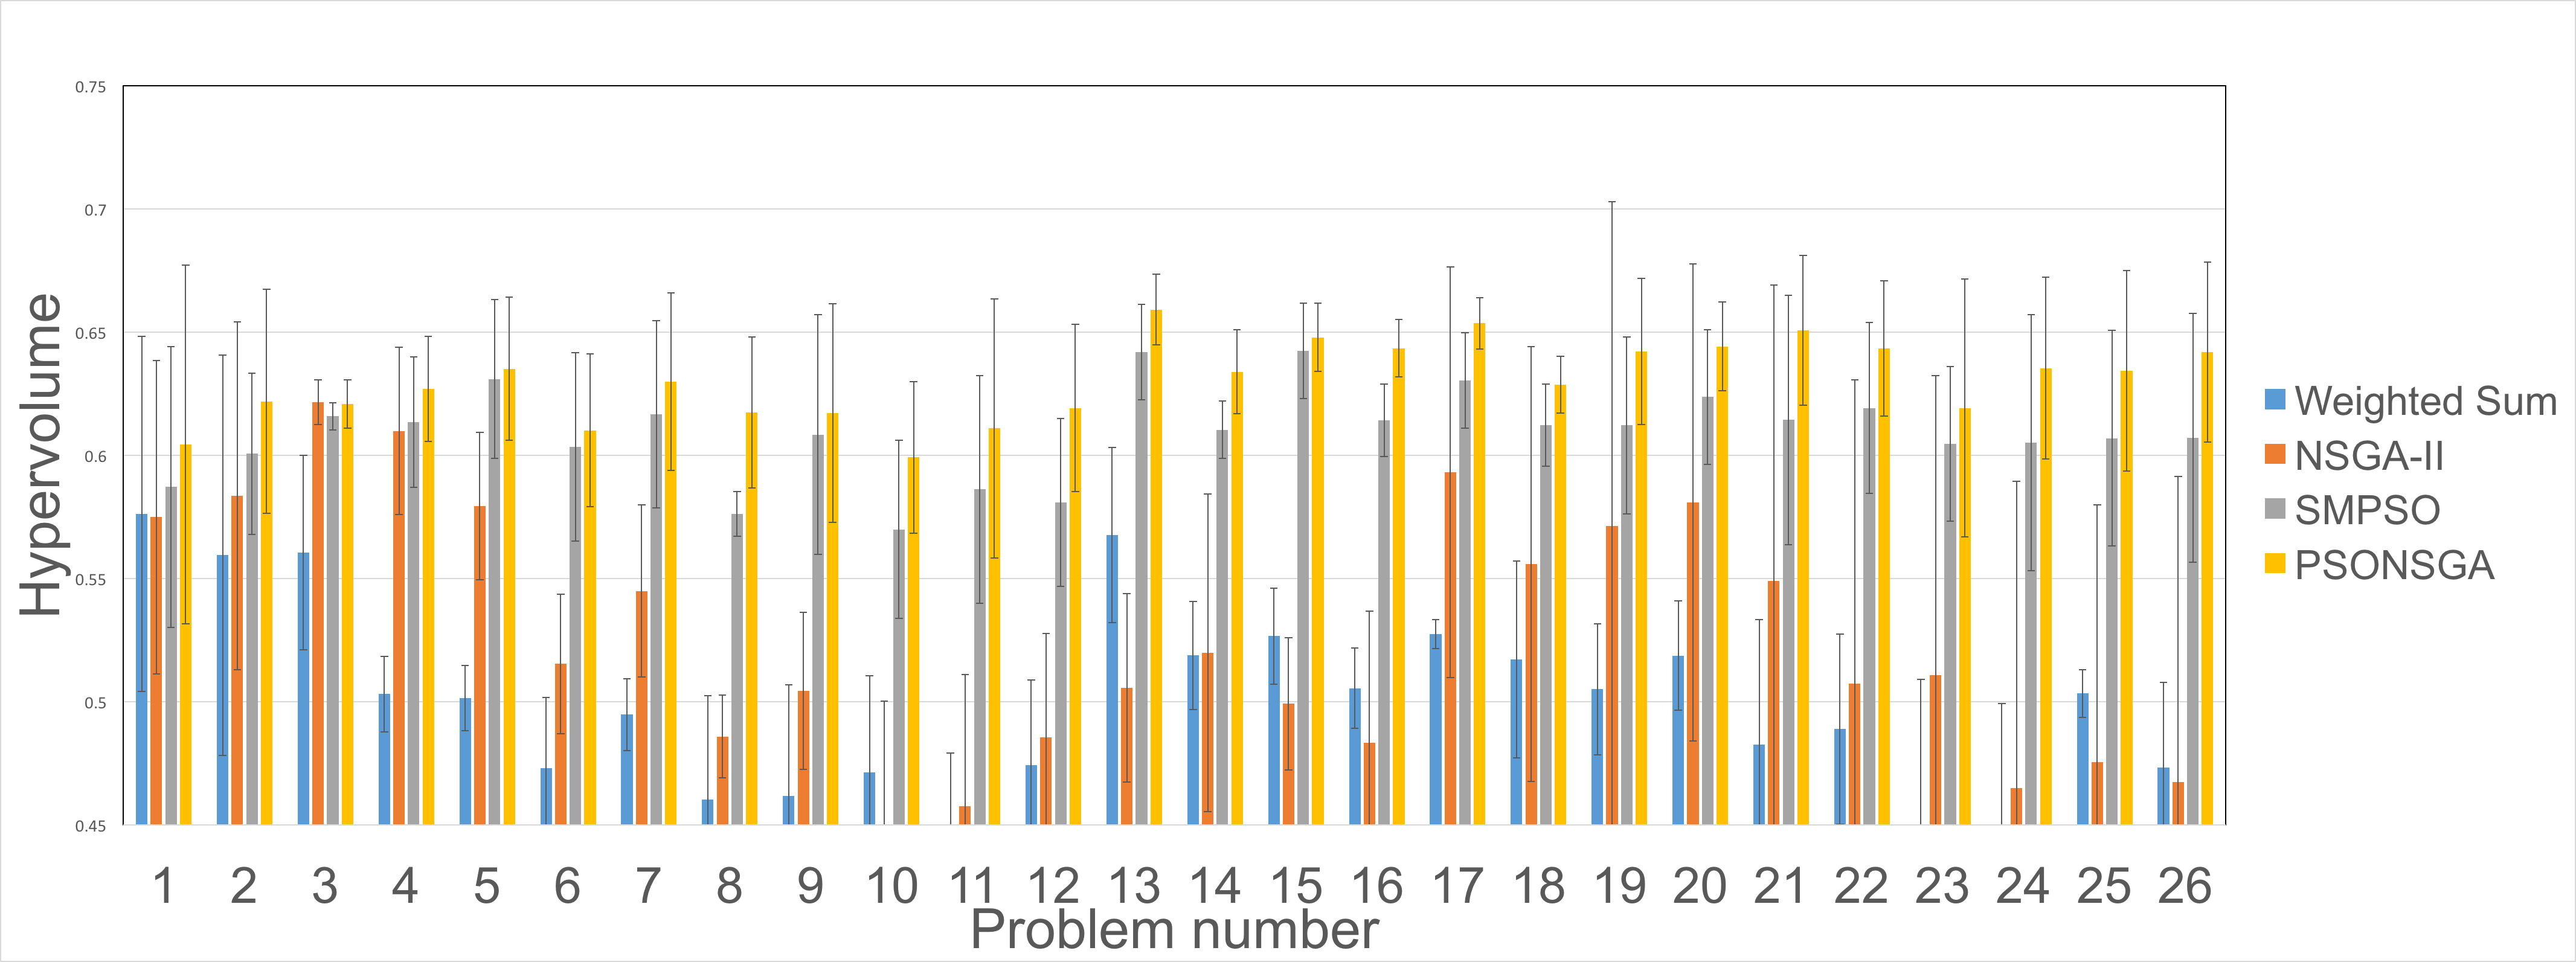
\includegraphics[page=1,width=\textwidth, height= 6cm]{hvaverageoverfour.png}}
\caption{HV indicator comparison (over four instance sets)} 
\label{hvaverage}
\end{figure*}

As shown in \Fig{hvaverage}, the PSONSGA algorithm achieves the best balance between convergence and diversity amongst the three evolutionary algorithms. The weighted sum approach produces worse HV values, because each individual branch and bound search can only produce one single solution. We can also notice that for large-scale problems, NSGA-II's HV values are worse than all three other algorithms. This is due to the larger search space in large-scale problems and the concentrated effect of the non-dominated sorting in the NSGA-II algorithm.


\subsubsection{IGD Indicator Comparison}
In this section, we examine the solution quality of the weighted sum, NSGA-II, SMPSO and PSONSGA algorithms by using the IGD quality indicator. The IGD indicator evaluates the quality of a solution set using a reference set. It generates the IGD value through calculating the average euclidean distance between the solution sets and the reference sets \cite{gaspar2015evolutionary}. %COMMENT: add a reference for IGD since this is the first you talk about it...

In our evaluation, we use the best non-dominated solutions returned by all three methods as the reference set. The IGD values for the four algorithms are presented in Table~\ref{table:igd}. The first column shows the problem number. Columns~2,~3,~4 and~5 display respectively, the average IGD value for the weighted sum, NSGA-II, SMPSO and PSONSGA. As can be seen, PSONSGA displays its superiority over the weighted sum method and the two existing evolutionary algorithms in this evaluation. The average IGD values for PSONSGA's solutions achieve the best IGD in 25 of the 26 problems. This improvement over NSGA-II and SMPSO can be explained by the information exchange between the PSO and GA phases in the PSONSGA procedure. This two-phase procedure has been proven to reach better Pareto front results as shown by the IGD indicator comparison.

\begin{table}[ht]
\caption{IGD indicator comparison (average over four instances)}\label{table:igd}
\centering
\begin{scriptsize}
\resizebox{\columnwidth}{!}{
\begin{tabular}{|*{5}{c|}}
\hline \textbf{Problem \#}&\textbf{Weighted sum}& \textbf{NSGA-II }& \textbf{SMPSO} &  \textbf{PSONSGA}\\
\hline
\hline
1 &$2.16E-01$&$1.01E-02$&$2.01E-03 $&\cellcolor{gray95}$1.43E-03$\\
2 &$1.31E-01$&$9.22E-03$&$2.09E-03 $&\cellcolor{gray95}$1.24E-03$\\
3 &$9.81E-02$&$4.95E-03$&$1.96E-03 $&\cellcolor{gray95}$1.11E-03$\\
4 &$4.11E-02$&$1.24E-02$&$2.46E-03 $&\cellcolor{gray95}$1.97E-03$\\
5 &$3.57E-02$&$1.30E-02$&$3.16E-03 $&\cellcolor{gray95}$3.02E-03$\\
6 &$3.57E-02$&$1.32E-02$&$3.55E-03 $&\cellcolor{gray95}$2.49E-03$\\
7 &$6.12E-02$&$1.17E-02$&$3.73E-03 $&\cellcolor{gray95}$2.81E-03$\\
8 &$9.72E-02$&$1.99E-02$&$3.68E-03 $&\cellcolor{gray95}$2.44E-03$\\
9 &$9.83E-02$&$1.79E-02$&$4.44E-03 $&\cellcolor{gray95}$3.28E-03$\\
10&$1.13E-01$&$1.73E-02$&$5.32E-03$&\cellcolor{gray95}$3.83E-03$\\
11&$1.34E-01$&$2.06E-02$&$4.98E-03$&\cellcolor{gray95}$3.52E-03$\\
12&$1.40E-01$&$2.08E-02$&$5.54E-03$&\cellcolor{gray95}$4.33E-03$\\
13&$4.47E-02$&$1.57E-02$&$2.37E-03$&\cellcolor{gray95}$1.48E-03$\\
14&$5.21E-02$&$1.78E-02$&$2.59E-03$&\cellcolor{gray95}$1.69E-03$\\
15&$7.05E-02$&$1.68E-02$&$2.40E-03$&\cellcolor{gray95}$1.69E-03$\\
16&$1.24E-01$&$1.70E-02$&$3.11E-03$&\cellcolor{gray95}$2.05E-03$\\
17&$1.18E-01$&$1.51E-02$&$3.53E-03$&\cellcolor{gray95}$2.53E-03$\\
18&$1.82E-01$&$1.70E-02$&$3.50E-03$&\cellcolor{gray95}$2.33E-03$\\
19&$1.70E-01$&$1.52E-02$&$3.32E-03$&\cellcolor{gray95}$2.59E-03$\\
20&$3.03E-01$&$1.76E-02$&$3.43E-03$&\cellcolor{gray95}$2.25E-03$\\
21&$2.62E-01$&$1.64E-02$&$3.86E-03$&\cellcolor{gray95}$3.00E-03$\\
22&$3.03E-01$&$1.92E-02$&$3.61E-03$&\cellcolor{gray95}$2.03E-03$\\
23&$3.48E-01$&$1.53E-02$&$3.66E-03$&\cellcolor{gray95}$2.78E-03$\\
24&$4.03E-01$&$1.97E-02$&$3.34E-03$&\cellcolor{gray95}$2.17E-03$\\
25&$3.68E-01$&$1.65E-02$&\cellcolor{gray95}$3.66E-03$&$3.97E-03$\\
26&$5.32E-01$&$1.93E-02$&$4.43E-03$&\cellcolor{gray95}$4.27E-03$\\\hline
\end{tabular}}
\end{scriptsize}
\end{table}


\subsubsection{Delay Gap Comparison}
Since we solved the weighted sum formulation with the CPLEX solver, each solution point from the CPLEX solver is an optimal solution. In other words, under the same expense condition, the traffic delay produced by the weighted sum and CPLEX can achieve the optimum. Using CPLEX solutions as the reference, we calculate the average delay gaps between CPLEX and the evolutionary algorithms. The average delay gaps were computed only if the same cost exists in the weighted sum solution sets and CPLEX has found the optimal solutions (the relative MIP equals to zero). 

Table~\ref{delaygapss} shows the statistical analysis for delay gaps over the four instance sets. The first three columns represent the minimum, the maximum, and the average delay gaps. The following two columns are the standard deviation and the 95\% confidence interval for the average delay gaps. As shown in Table~\ref{delaygapss}, without considering the diversity and distribution in the solution sets, NSGA-II gives the best delay gaps to optimal solutions. The reason behind this is the non-dominated sorting in NSGA-II concentrates the solution sets towards the optimal front. However, this sorting process sacrifices the solution diversity for a better convergence quality. This is the same reason why the solutions produced by the NSGA-II algorithm provide worse HV values. PSONSGA achieves the second best among the three evolutionary algorithms.

\begin{table}[ht]
\centering
\caption{Delay gap comparison (over four instance sets)}\label{delaygapss}
\resizebox{\columnwidth}{!}{
\begin{tabular}{|*{7}{c|}}
\hline
\textbf{Algorithms}& \textbf{Min.gap} & \textbf{Max.gap }&\textbf{Ave.gap} &\textbf{Std.dev}&\textbf{95\% C.I.}\\
&\textbf{(\%)} &\textbf{(\%)}&\textbf{(\%)}&\textbf{(\%)}&\textbf{(\%)}\\
\hline
 NSGA-II&0.00&7.80&0.30&0.81&0.30$\pm$0.15\\
SMPSO&0.00&8.50&0.60&1.19&0.60$\pm$0.22\\
PSONSGA&0.00&7.80&0.50&1.12&0.50$\pm$0.21\\
\hline
\end{tabular}}
\end{table}


\subsubsection{CPU Time Comparison}
\Fig{cputimeover4} provides the comparison in terms of the CPU time between the weighted sum method and the three evolutionary algorithms over the four instance sets with a 95\% confidence interval. 

As shown in \Fig{cputimeover4}, all three evolutionary algorithms can provide good quality Pareto frontier in a reasonable amount of time. For small-scale problems (problems 1 to 12), the three evolutionary algorithms can finish the optimization within 30 seconds. For large-scale problems, evolutionary algorithms' solution times are still within a reasonable range. For example, to solve problem 26 (instance-1), NSGA-II, SMPSO, PSONSGA, each respectively took 5,303 seconds, 1,639 seconds and 5,464 seconds. In comparison, the weighted sum method using the CPLEX solver takes 19,510 seconds, which is approximately 3.5 times longer than PSONSGA. We also notice that, although fast for small size problems, CPLEX's CPU time is almost increasing exponentially with respect to the problem size. This corresponds with the fact that the fog planning problem is NP-hard as described before.

\begin{figure*}[ht]
\centerline{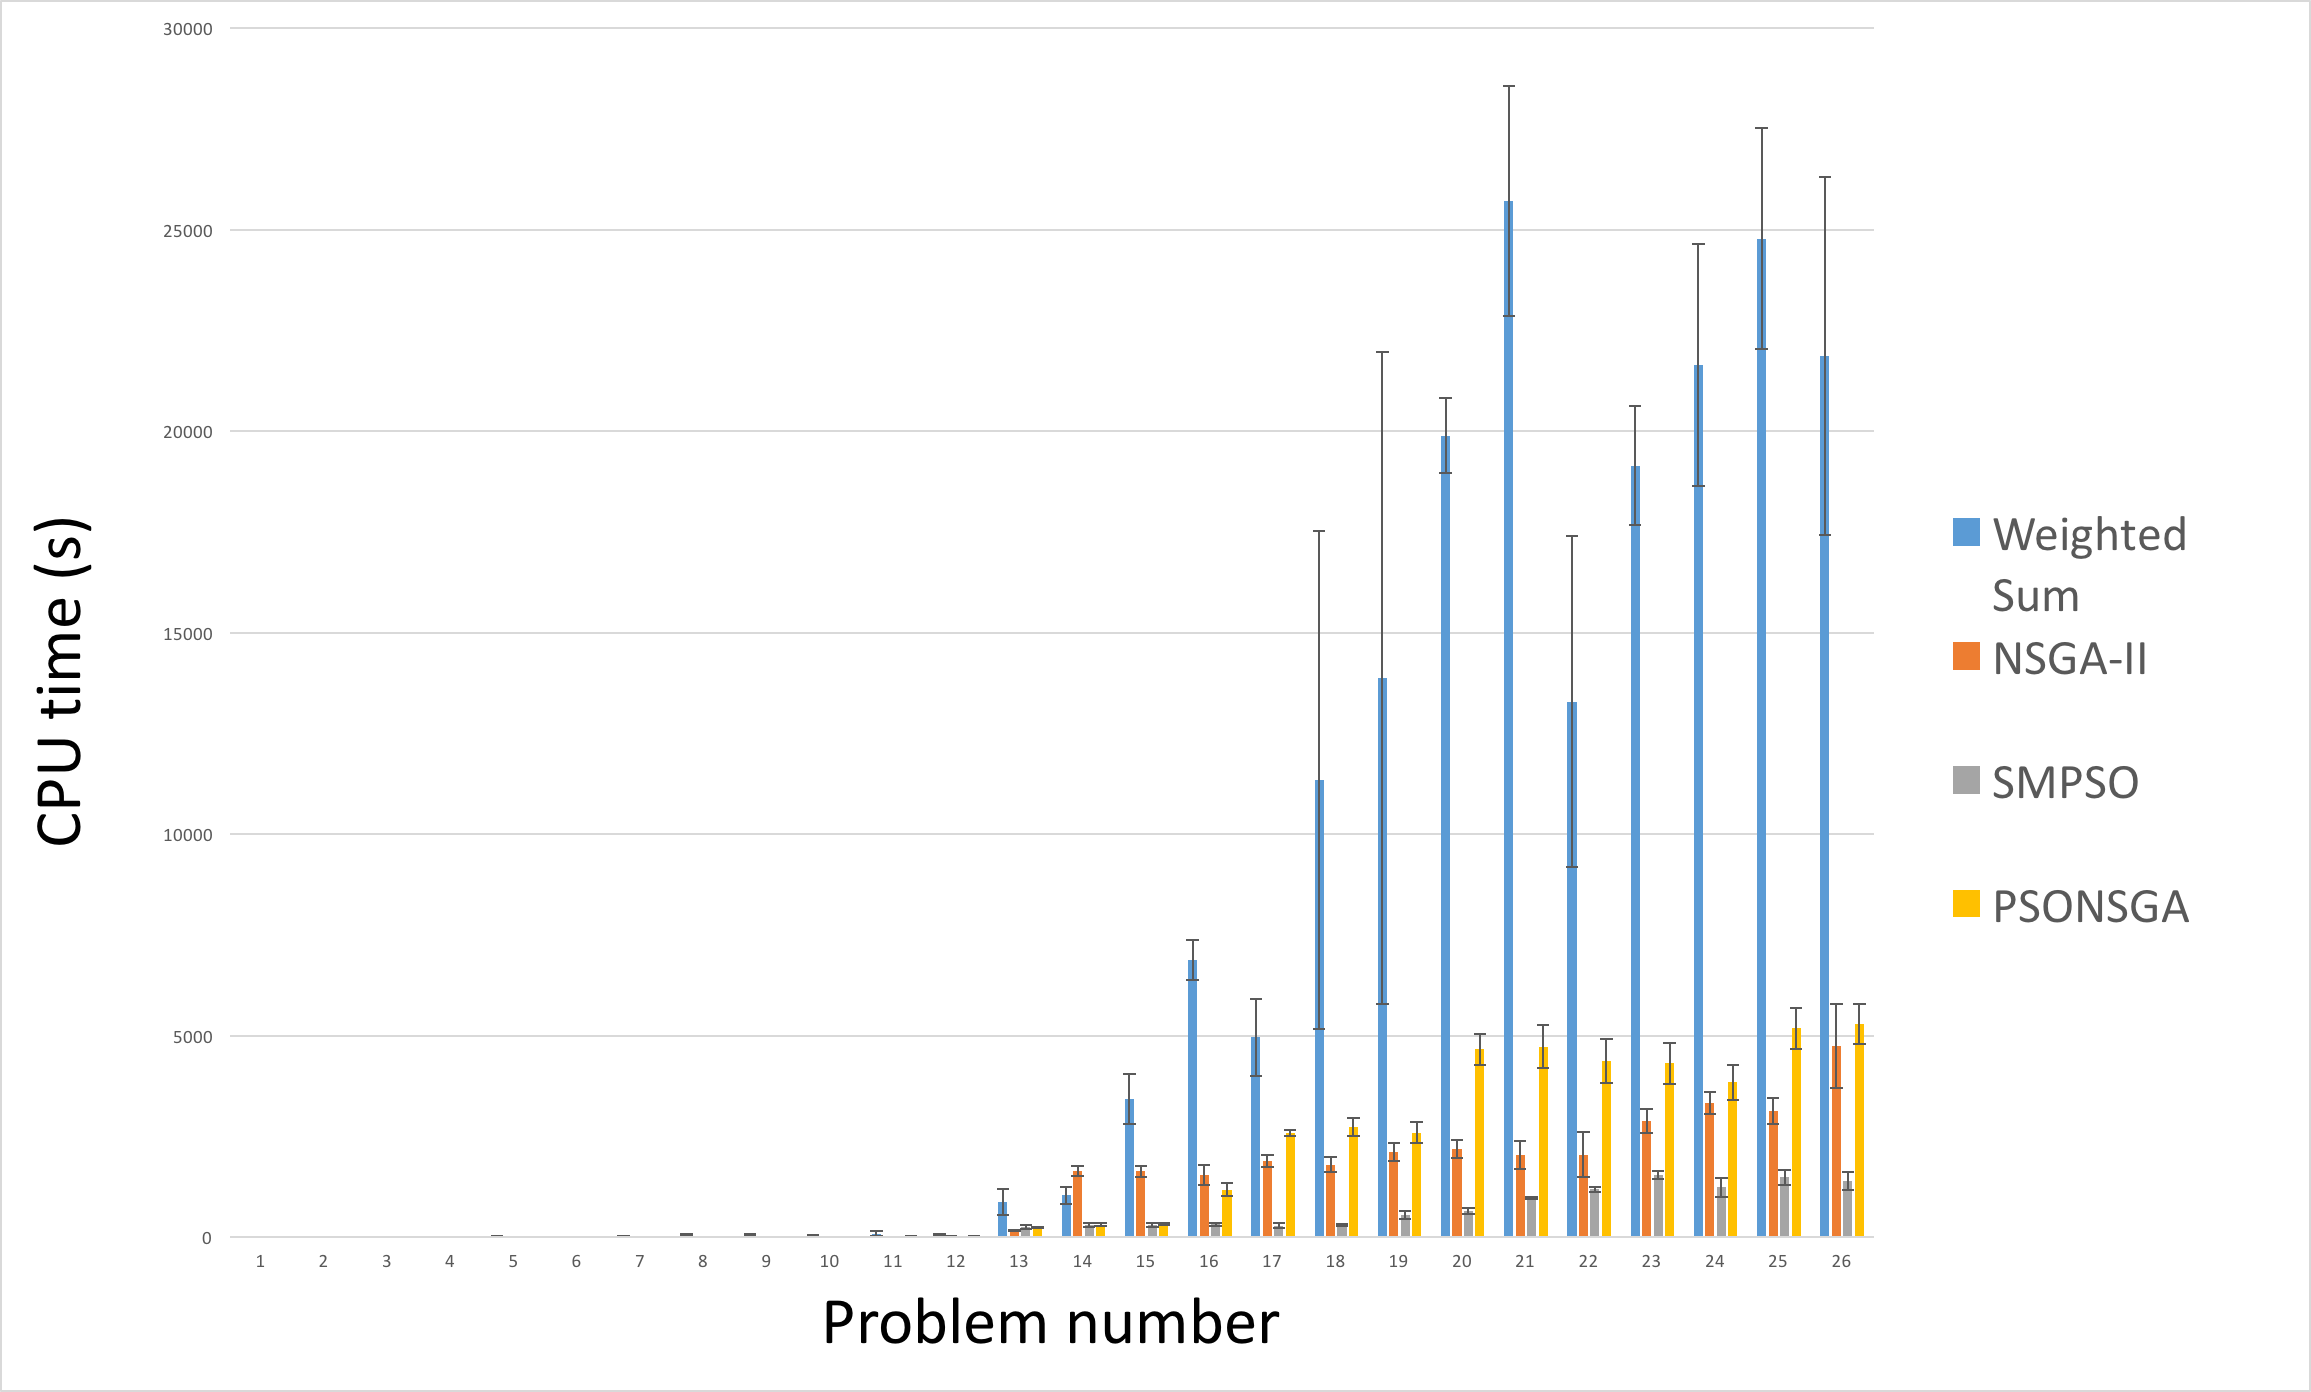
\includegraphics[page=1,width=\textwidth,height=6cm]{cputimeover4}}
\caption{CPU time comparison (over four instance sets)} 
\label{cputimeover4}
\end{figure*}

From the delay gap comparison shown in Table~\ref{delaygapss} and the CPU time comparison in \Fig{cputimeover4}, we can conclude that the evolutionary algorithms are able to use less CPU time to generate close to optimal solutions. At the same time, PSONSGA attains a good balance between the solution convergence and diversity, compared to the two existing algorithms (NSGA-II and SMPSO).


\section{Related Works}\label{relwork}
Fog computing research has attracted lots of attention. Researchers have been working on studies of fog architecture~\cite{fcsmartcity}, fog communication protocols~\cite{Peng:2016:FRA:3029494.3029575} and application logic in fog networks~\cite{SUN2017687}. Regarding workload allocation and resource management in fog computing networks, Dsouza et al.~\cite{secme} proposed a policy-based resource management in fog computing, which expanded the current fog computing platform to support collaboration and interoperability between different resources. Deng et al., in~\cite{fcworkload}, focused on investigating the tradeoff between power consumption and transmission delay in the fog-cloud computing system, and they formulated a work-load allocation problem that aims at minimal power consumption considering the constrained service delay. Sun and Zhang~\cite{SUN2017687} proposed a fog computing structure to integrate spare resources in the network applying a crowd-funding algorithm.



%Among all the work describe above that are directly focusing on the fog computing environment, none of them addresses the planning and design of fog networks as we are presenting it in this paper. 
%%%%REVISED update the references
Hua-Jun et al.~\cite{hong2016dynamic} surveyed the existing platforms, virtualization technologies and approaches to implement the fog computing platform. The optimizing model they proposed focused on maximizing the computation offloading, but failed to consider the network performance in resource allocation process, and the incurred costs in computing platform construction.
Bachmann et al.~\cite{bachmann2017design} proposed a fog computing framework. This framework mplemented the major functionalities of a fog computing architecture. From the perspective of software engineering, this research can be a good starting point of the future research in fog computing and service deployment.
Haider F et al.~\cite{haider2017planning} proposed a multi-objective model for the fog network planning. The model attempted to jointly optimized the network traffic and network delay. However, this model failed to consider the influence of the budget in network construction and the model could be reduced to a single-objective model.
Liu et al.~\cite{liu2018tensor} proposed a customized optimization framework for the fog network, in which the optimization objectives can be arbitrarily combined. Compared to the heuristic algorithm, the tensor-based representation and computation model employed in this paper hugely complicated the optimization process and the time complexity of this method is unmanageable.
Another closely related topic under the network planning context is the distributed-cloud planning. 
Hwang et al.~\cite{hwang2013distributed} illustrated the planning processes of creating high-performance, scalable, reliable distributed computing systems including the design principles, architectures, and innovative applications. 
Khosravi and Buyya~\cite{enerfoot} presented a taxonomy and classification of the existing techniques for resource management in achieving a green cloud computing environment. 
Iturriaga et al.~\cite{ITOR:ITOR12294} studied the application of multi-objective evolutionary algorithms for solving the energy-aware scheduling problem. The scheduling problem took account of the scheduling of large workflows in a federation of datacenters. In another study, Xu and Li, in~\cite{6566873}, presented a joint request mapping and response routing policy for geo-distributed cloud services. The utility functions were used to capture the performance goals. However, their model focused on the resource mapping and traffic routing in distributed cloud networks without considering the placement and sizing of the geo-distributed cloud. 
Among all the work describe above that are directly related to the distributed-cloud planning, none of them addresses the facility planning and provisioning in distributed computing networks as we are presenting it in this paper.

%COMMENT: You should mention one more time that a recent survey paper confirms that work on the planning of fog netowrks is important but still lacking...this is good for us...

In particular, the recent comprehensive survey \cite{mouradian2017comprehensive} in fog research has confirmed that work on the planning and design of fog system deployment is vital but still lacking detailed research so far.

\section{Conclusion}\label{conclu}
In this paper, we first proposed a multi-objective modular facility location model for planning fog networks. The multi-objective combinatorial model enables us to fully explore the searching domain with different fog location selection, fog type selection and user allocation combinations. The model produces the Pareto front solution set over two objectives: the network delay and the capital expenditure. Decision makers can use this Pareto front to make reliable decision on fog infrastructure building plan. 

We also apply one exact algorithm (weighted sum) and three heuristic algorithms (NSGA-II, SMPSO and PSONSGA) to solve the model. The results from these algorithms are compared in terms of the HV indicator, IGD indicator and delay gaps. The experimental results confirm that evolutionary algorithms can be notably efficient in execution time compared to the weighted sum-based approach. In terms of the HV and IGD indicator, PSONSGA achieves the best HV and IGD values for most of the problem sizes. In contrast, NSGA-II was able to return good solutions in terms of the delay objective value without considering the diversity and coverage of solution frontiers.

In the real world of fog planning, the number of edge-clusters can be extremely large, and the network topology, conditions and restrictions will be more complicated. Therefore, using the weighed sum method and CPLEX can be time-consuming. In fact, the proposed algorithm can be more appropriate in this situation. PSONSGA is recommended for solving the fog planning problem as it achieves the best balance between the solution diversity, convergence and computation time.

In future, our model can be further extended to a dynamic expansion model in which existing fog facility can be partially closed and reopened later based on on-demand traffic. The fog site can be relocated to accommodate seasonal traffic changes. PSONSGA can be used as a starting point for this extension. Considering its high solution time efficiency, PSONSGA can be even promising on this problem, especially, because the dynamic model problem with time periods could easily scale up. In this context, the exact algorithm such as the weighted sum is struggling to produce results.





% if have a single appendix:
%\appendix[Proof of the Zonklar Equations]
% or
%\appendix  % for no appendix heading
% do not use \section anymore after \appendix, only \section*
% is possibly needed

% use appendices with more than one appendix
% then use \section to start each appendix
% you must declare a \section before using any
% \subsection or using \label (\appendices by itself
% starts a section numbered zero.)
%





%%\fi

% Can use something like this to put references on a page
% by themselves when using endfloat and the captionsoff option.
\ifCLASSOPTIONcaptionsoff
  \newpage
\fi



% trigger a \newpage just before the given reference
% number - used to balance the columns on the last page
% adjust value as needed - may need to be readjusted if
% the document is modified later
%\IEEEtriggeratref{8}
% The "triggered" command can be changed if desired:
%\IEEEtriggercmd{\enlargethispage{-5in}}

% references section

% can use a bibliography generated by BibTeX as a .bbl file
% BibTeX documentation can be easily obtained at:
% http://mirror.ctan.org/biblio/bibtex/contrib/doc/
% The IEEEtran BibTeX style support page is at:
% http://www.michaelshell.org/tex/ieeetran/bibtex/
\bibliographystyle{IEEEtran}
% argument is your BibTeX string definitions and bibliography database(s)
\bibliography{IEEEabrv,decheng}
%
% <OR> manually copy in the resultant .bbl file
% set second argument of \begin to the number of references
% (used to reserve space for the reference number labels box)
%\begin{thebibliography}{1}

%\bibitem{IEEEhowto:kopka}
%H.~Kopka and P.~W. Daly, \emph{A Guide to \LaTeX}, 3rd~ed.\hskip 1em plus
 % 0.5em minus 0.4em\relax Harlow, England: Addison-Wesley, 1999.

%\end{thebibliography}

% biography section
% 
% If you have an EPS/PDF photo (graphicx package needed) extra braces are
% needed around the contents of the optional argument to biography to prevent
% the LaTeX parser from getting confused when it sees the complicated
% \includegraphics command within an optional argument. (You could create
% your own custom macro containing the \includegraphics command to make things
% simpler here.)
%\begin{IEEEbiography}[{\includegraphics[width=1in,height=1.25in,clip,keepaspectratio]{mshell}}]{Michael Shell}
% or if you just want to reserve a space for a photo:



% if you will not have a photo at all:
\begin{IEEEbiography}
[{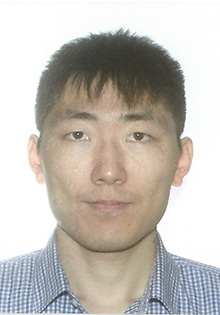
\includegraphics[width=1in,height=1.25in,clip,keepaspectratio]{Decheng}}]{Decheng Zhang}
received his Bachelor of Engineering degree from the Department of Information and Communication Engineering, Beijing University of Posts and Telecommunications, China, in 2013. He received his Master of Applied Science degree from the Department of Systems and Computer Engineering at the Carleton University, Canada, in 2018. His research interests include fog/edge computing, fog network planning, optimization research and cloud computing.
\end{IEEEbiography}

\begin{IEEEbiography}
[{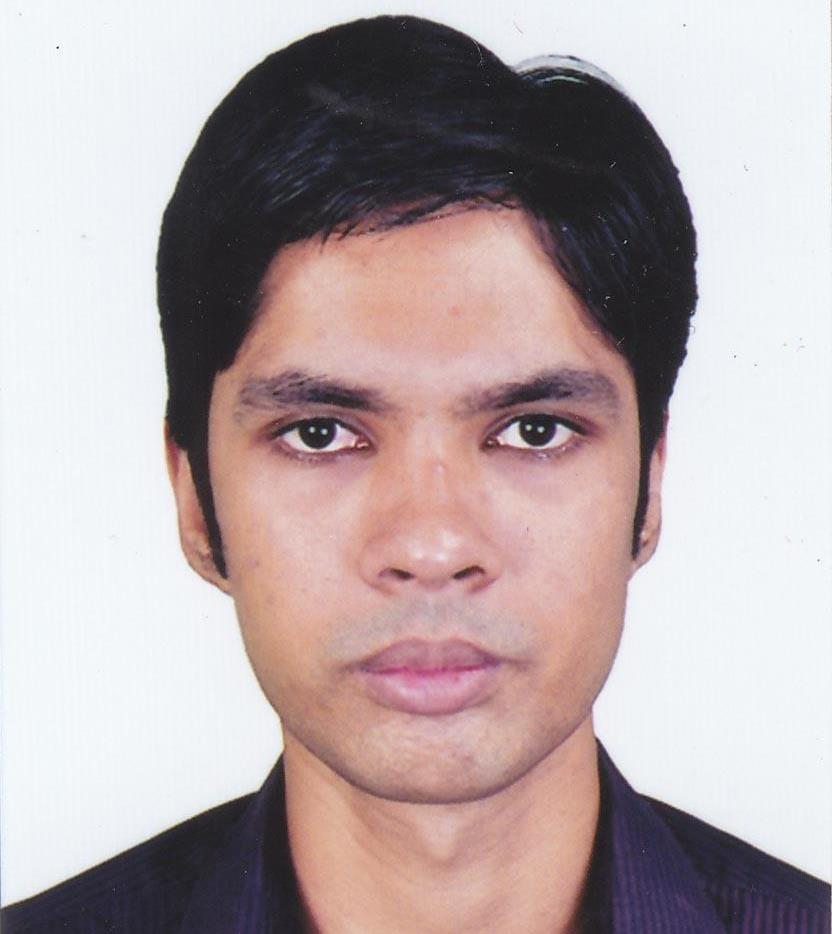
\includegraphics[width=1in,height=1.25in,clip,keepaspectratio]{Faisal}}]{Faisal Haider}
received his Bachelor of Science degree in Electrical and Electronics Engineering from American International University-Bangladesh in 2013. He received his Master of Applied Science degree from the Department of Systems and Computer Engineering from Carleton University, Canada, in 2018. His research interests include fog/edge computing, network planning and design, network optimization and cloud computing.
\end{IEEEbiography}




\begin{IEEEbiography}
[{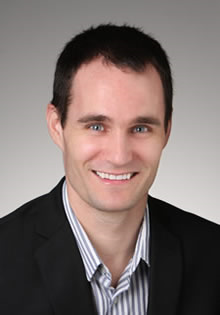
\includegraphics[width=1in,height=1.25in,clip,keepaspectratio]{ProfMarc}}]{Marc St-Hilaire}
joined Carleton University in 2006 upon completion of his PhD in Computer Engineering, from \'Ecole Polytechnique of Montr\'eal. He is currently an associate professor with the School of Information Technology with a cross appointment with the Department of Systems and Computer Engineering at Carleton University. Dr. St-Hilaire is conducting research on various aspects of wireline and wireless communication systems. More precisely, he is interested in network planning and infrastructure, network protocols, network interconnection, and performance analysis. With more than 110 publications, his work has been published in several journals and international conferences. Finally, Dr. St-Hilaire is actively involved in the research community. In addition to serving as a member of technical program committees of various conferences, he is equally involved in the organization of several national and international conferences and workshops. He is also a senior member of the IEEE.
\end{IEEEbiography}

\begin{IEEEbiography}
[{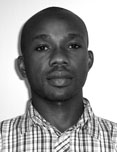
\includegraphics[width=1in,height=1.25in,clip,keepaspectratio]{DrMakaya}}]{Christian Makaya}
is currently a researcher at IBM T.J. Watson Research Center, NY, USA. Prior to joining IBM, he was a senior research scientist at Telcordia Technologies, NJ, USA and a visiting researcher at Ericsson Research, Montreal, Canada. His work has been a catalyst behind several new initiatives and technologies resulting in delivery of high-value capabilities to products and services. For his technical contributions, he has been recognized by several high-prestige internal awards by IBM. Dr. Makaya leads several technical research activities in the areas of distributed systems and analytics with the mission of delivering deep technical breakthroughs. The focus of his current research interests is on distributed AI and ML, edge computing, Internet of Things (IoT), network functions virtualization (NFV), policy-based management systems, and cyber-security. Dr. Makaya has authored numerous technical papers in peer-reviewed journals and conferences, and filled several patents. He received his Ph.D. in Computer Engineering from Polytechnique Montreal (2007). Dr. Makaya is an active member and volunteer of IEEE and serves on the Industry Outreach Board of IEEE Communication Society (ComSoc). He served as the co-chair of IEEE Young Professionals for the IEEE Princeton/Central Jersey Section.
\end{IEEEbiography}


% insert where needed to balance the two columns on the last page with
% biographies
%\newpage



% You can push biographies down or up by placing
% a \vfill before or after them. The appropriate
% use of \vfill depends on what kind of text is
% on the last page and whether or not the columns
% are being equalized.

%\vfill

% Can be used to pull up biographies so that the bottom of the last one
% is flush with the other column.
%\enlargethispage{-5in}



% that's all folks
\end{document}


